%=============================================================================
% Uncertainty-Aware Machine Learning for Microwave-Based Body Composition
% Assessment
%
% Author  : Abhishek Yadav
% Uppsala University — Master's Thesis, May 2026
%
% Compile:  pdflatex thesis.tex  (two passes for cross-references)
%           pdflatex thesis.tex
%=============================================================================

\documentclass[12pt, a4paper, oneside]{report}

%--- Encoding & Language ------------------------------------------------------
\usepackage[utf8]{inputenc}
\usepackage[T1]{fontenc}
\usepackage[english]{babel}

%--- Page Layout --------------------------------------------------------------
\usepackage[
  top=2.5cm, bottom=2.5cm,
  left=3.0cm, right=2.5cm,
  headheight=15pt
]{geometry}

%--- Typography ---------------------------------------------------------------
\usepackage{lmodern}
\usepackage{microtype}
\usepackage{setspace}
\onehalfspacing

%--- Mathematics --------------------------------------------------------------
\usepackage{amsmath}
\usepackage{amssymb}
\usepackage{bm}

%--- Figures ------------------------------------------------------------------
\usepackage{graphicx}
\usepackage{float}
\usepackage{subcaption}
\usepackage{caption}
\captionsetup{font=small, labelfont=bf, width=0.96\textwidth}
\captionsetup[subfigure]{font=small, labelfont=bf}
\setlength{\belowcaptionskip}{4pt}
\setlength{\abovecaptionskip}{8pt}
\graphicspath{{figures/}}

%--- Tables -------------------------------------------------------------------
\usepackage{booktabs}
\usepackage{multirow}
\usepackage{array}
\usepackage{tabularx}
\newcolumntype{C}{>{\centering\arraybackslash}X}

%--- Header / Footer ----------------------------------------------------------
\usepackage{fancyhdr}
\pagestyle{fancy}
\fancyhf{}
\fancyhead[L]{\small\leftmark}
\fancyhead[R]{\small\thepage}
\renewcommand{\headrulewidth}{0.4pt}
\fancypagestyle{plain}{%
  \fancyhf{}
  \fancyfoot[C]{\thepage}
  \renewcommand{\headrulewidth}{0pt}
}

%--- Colours ------------------------------------------------------------------
\usepackage[dvipsnames]{xcolor}
\definecolor{uppsalared}{RGB}{153,0,0}

%--- Hyperlinks ---------------------------------------------------------------
\usepackage[
  colorlinks=true,
  linkcolor=uppsalared,
  citecolor=uppsalared,
  urlcolor=MidnightBlue,
  bookmarks=true,
  pdftitle={Uncertainty-Aware Machine Learning for Microwave-Based Body Composition Assessment},
  pdfauthor={Abhishek Yadav}
]{hyperref}

%--- Miscellaneous ------------------------------------------------------------
\usepackage{enumitem}
\usepackage{eurosym}        % \euro symbol

%--- Chapter style ------------------------------------------------------------
\usepackage{titlesec}
\titleformat{\chapter}[display]
  {\normalfont\Large\bfseries\color{uppsalared}}
  {\chaptertitlename\ \thechapter}{12pt}{\LARGE}
\titlespacing*{\chapter}{0pt}{0pt}{20pt}

%=============================================================================
\begin{document}
%=============================================================================

%--- Title Page ---------------------------------------------------------------
\begin{titlepage}
  \centering
  \vspace*{1cm}

  {
\includegraphics[width=0.35\textwidth]{uu_logo}\par}\vspace{0.5cm}
  {\color{uppsalared}\rule{\textwidth}{1.5pt}\par}
  \vspace{1cm}

  {\LARGE\bfseries Uncertainty-Aware Machine Learning\\[6pt]
   for Microwave-Based Body Composition\\[6pt]
   Assessment\par}

  \vspace{1.2cm}
  {\large\itshape Abhishek Yadav\par}
  \vspace{0.4cm}
  {\normalsize
    Department of Electrical Engineering\\
    Uppsala University\\
    Sweden\par}

  \vfill

  \begin{tabular}{ll}
    \textbf{Supervisor:} & Bappaditya Mandal \\[4pt]
    \textbf{Reviewer:}   & Robin Augustine   \\[4pt]
    \textbf{Programme:}  & Master's in Embedded Systems / Electrical Engineering \\[4pt]
    \textbf{Date:}       & May 2026
  \end{tabular}

  \vspace{1cm}
  {\color{uppsalared}\rule{\textwidth}{1.5pt}\par}
\end{titlepage}

%--- Front Matter -------------------------------------------------------------
\pagenumbering{roman}

%--- Abstract -----------------------------------------------------------------
\chapter*{Abstract}
\addcontentsline{toc}{chapter}{Abstract}

Non-invasive body composition assessment---the quantification of skin, subcutaneous fat, and muscle tissue thickness from external measurements---is a clinically valuable capability that currently requires expensive imaging equipment or trained operators. Microwave sensing offers a low-cost, portable, and non-contact alternative: by measuring the reflection and transmission of radio-frequency signals in the 1--3\,GHz range against a body surface, one can extract information about the dielectric properties and geometric arrangement of underlying tissue layers. However, prior machine learning work on microwave-based body composition has reported only point predictions, providing no indication of predictive confidence. A clinician who receives a prediction of ``Fat $=$ 11.3\,mm'' with no associated uncertainty cannot determine whether to trust that figure, making the output of limited practical value.

This thesis introduces uncertainty-aware machine learning models for the MAS (Microwave Assessment of Sarcopenia) Volunteer Study dataset, consisting of S-parameter measurements from 16 training volunteers (September 2022, $n=431$ samples) and 23 independent validation volunteers (March 2023, $n=471$ samples). We implement and evaluate two probabilistic regression approaches---Monte Carlo Dropout and Deep Ensembles---both employing a heteroscedastic Gaussian negative log-likelihood training objective that enables the network to jointly predict tissue thickness and calibrate its own predictive uncertainty. Deterministic baselines (Random Forest, XGBoost, FCNN) are evaluated under 4-fold volunteer-level GroupKFold cross-validation.

On the independent March 2023 cohort, MC Dropout achieves Expected Calibration Error (ECE) values of 0.074 (skin), 0.094 (fat), and 0.020 (muscle), indicating that stated confidence levels closely match empirically observed coverage. A clinical risk-score system based on the total predictive standard deviation $\sigma_{\mathrm{total}}$ achieves RMSE separation ratios of 1.026--1.060$\times$ across all targets, confirming that high-uncertainty predictions have genuinely higher prediction error. Deterministic baselines achieve prediction interval coverage probability (PICP) of exactly zero and negative log-likelihood values in the tens of thousands, confirming they provide no clinically usable probabilistic output.

We conclude that calibrated uncertainty quantification is not a theoretical refinement but a functional prerequisite for deploying microwave-based body composition sensing in clinical settings. A system that can identify its own unreliable predictions and redirect those cases to confirmatory ultrasound is qualitatively more useful than a system offering confident but untrustworthy point estimates.

\vspace{1em}
\noindent\textbf{Keywords:} microwave sensing, S-parameters, body composition, uncertainty quantification, Monte Carlo Dropout, Deep Ensembles, heteroscedastic regression, Expected Calibration Error, sarcopenia.

%--- Acknowledgements ---------------------------------------------------------
\chapter*{Acknowledgements}
\addcontentsline{toc}{chapter}{Acknowledgements}

I would like to thank my supervisor, Bappaditya Mandal, for his guidance throughout this project, and my reviewer, Robin Augustine, for his valuable feedback. I am grateful to Viktor Mattsson for providing access to the MAS Volunteer Study datasets and for his thorough documentation of the measurement protocol. Finally, I thank the volunteer participants whose measurements made this research possible.

%--- Table of Contents --------------------------------------------------------
\tableofcontents

%--- List of Figures ----------------------------------------------------------
\listoffigures
\addcontentsline{toc}{chapter}{List of Figures}

%--- List of Tables -----------------------------------------------------------
\listoftables
\addcontentsline{toc}{chapter}{List of Tables}

%=============================================================================
\pagenumbering{arabic}
%=============================================================================

%=============================================================================
\chapter{Introduction}
\label{ch:intro}
%=============================================================================

\section{Clinical Motivation}

Body composition---the quantitative breakdown of the human body into its constituent tissue types---is a medically significant parameter across a wide range of clinical contexts. The relative proportions of skin, subcutaneous adipose tissue, and skeletal muscle influence metabolic rate, surgical outcomes, and serve as key indicators for conditions ranging from obesity and metabolic syndrome to sarcopenia and malnutrition. Sarcopenia, the progressive loss of skeletal muscle mass and function associated with ageing, is particularly relevant: it is associated with increased risk of falls, hospitalisation, and mortality in older adults, and timely identification allows interventions that substantially improve patient outcomes~\cite{sergi2016}.

The current gold standard for regional body composition assessment at the tissue level is B-mode diagnostic ultrasound, which provides real-time cross-sectional images of tissue layers with millimetre-level precision and no ionising radiation. However, ultrasound has significant practical limitations as a population-scale screening tool. Equipment costs range from \euro{}10{,}000 to \euro{}100{,}000; the technique requires a trained sonographer to position the probe, interpret artefacts, and apply anatomical judgement; and equipment is typically clinic-fixed, precluding deployment in nursing homes, rehabilitation centres, or remote settings.

Dual-energy X-ray absorptiometry (DEXA) provides whole-body composition estimates with high accuracy but involves radiation exposure and is available only in specialised facilities. Bioelectrical impedance analysis (BIA) is cheap and portable but provides only coarse whole-body estimates with limited sensitivity to local tissue changes.

Microwave sensing represents a qualitatively different approach. A compact antenna placed against the skin radiates low-power electromagnetic signals in the 1--3\,GHz range. The reflected signal (S11) and transmitted signal (S21) carry information about the dielectric properties of the tissue layers beneath the sensor. Different tissues have markedly different dielectric permittivities at these frequencies: skin has high water content and high permittivity, fat has low water content and low permittivity, and muscle has intermediate properties. A single vector network analyser (VNA) such as the nanoVNA costs approximately \euro{}50--100, is battery-operable, and requires no special training to position against the body---properties that make microwave sensing highly attractive for point-of-care screening.

\section{The Clinical Translation Gap}

Several prior studies have demonstrated that machine learning models trained on S-parameter data can achieve statistically significant correlations with tissue thickness measurements~\cite{mattsson2022,sensors21}. However, nearly all published work has framed the problem as a \emph{deterministic} regression task: given an input spectrum, output a single point estimate for each tissue parameter. This framing is clinically inadequate.

Consider: a microwave sensor outputs ``Fat $= 11.3$\,mm''. If the model's true error is $\pm 1$\,mm, this figure is actionable. If the error is $\pm 8$\,mm, it may be nearly meaningless---spanning the full range from lean to obese. Without an uncertainty estimate, the clinician cannot distinguish these cases, and the output is actively misleading.

Uncertainty quantification (UQ) closes this gap in three practically important ways:
\begin{enumerate}[noitemsep]
  \item \textbf{Calibrated intervals} allow the clinician to immediately assess whether a measurement is precise enough to inform a decision.
  \item \textbf{Automatic triage} lets the system accept confident predictions and redirect uncertain cases to ultrasound confirmation, preserving the economic benefit of screening.
  \item \textbf{Probabilistic output} is a prerequisite for any downstream Bayesian decision procedure, such as tracking changes in muscle mass over time.
\end{enumerate}

\section{Research Questions}

This thesis addresses three research questions:

\begin{description}
  \item[RQ1] Can machine learning models trained on S-parameter spectra predict skin, fat, and muscle thickness on previously unseen volunteers?
  \item[RQ2] Do Bayesian uncertainty methods (MC Dropout, Deep Ensembles) produce calibrated uncertainty estimates---i.e., do their confidence intervals contain the true value at the stated rate on an independent cohort?
  \item[RQ3] Can the predictive uncertainty serve as a reliable clinical risk flag, such that high-uncertainty predictions have genuinely higher prediction error?
\end{description}

\section{Contributions}

The principal contributions of this thesis are:
\begin{itemize}[noitemsep]
  \item First application of heteroscedastic MC Dropout and Deep Ensembles to the MAS Volunteer Study dataset.
  \item Volunteer-level evaluation strategy preventing data leakage (GroupKFold cross-validation and temporally separated test cohort).
  \item Full calibration analysis (ECE, PICP, MPIW, reliability diagrams) on an independent March 2023 cohort of 23 volunteers.
  \item A clinical risk-score system that flags predictions with $\sigma_{\mathrm{total}}$ above a threshold and demonstrates superior accuracy on the retained low-risk subset.
\end{itemize}

\section{Thesis Outline}

Chapter~\ref{ch:background} reviews the relevant background on microwave S-parameter sensing, body composition assessment, machine learning, and uncertainty quantification. Chapter~\ref{ch:data} describes the MAS dataset and the data preprocessing pipeline. Chapter~\ref{ch:features} covers feature engineering. Chapter~\ref{ch:models} presents all model architectures in full. Chapter~\ref{ch:results} reports experimental results. Chapter~\ref{ch:risk} describes the clinical risk-score system. Chapter~\ref{ch:discussion} discusses the findings and limitations. Chapter~\ref{ch:conclusion} concludes.

%=============================================================================
\chapter{Background and Related Work}
\label{ch:background}
%=============================================================================

\section{Microwave S-Parameters and Tissue Sensing}

A vector network analyser (VNA) stimulates a device under test with swept-frequency RF signals and measures the complex ratio of reflected and transmitted power. The resulting S-parameter matrix entries are:
\begin{equation}
  S_{11}(f) = \frac{V_1^-}{V_1^+}\bigg|_{V_2^+=0}, \qquad
  S_{21}(f) = \frac{V_2^-}{V_1^+}\bigg|_{V_2^+=0}
\end{equation}
where $V^+$ and $V^-$ denote incident and reflected voltage waves at each port. $S_{11}$ characterises reflection at the sensor surface (dominated by the skin--air interface and the dielectric loading of sub-surface tissue), while $S_{21}$ characterises transmission through all intervening layers. The Touchstone S2P file format stores these measurements as rows of (frequency, $\mathrm{Re}[S_{11}]$, $\mathrm{Im}[S_{11}]$, $\mathrm{Re}[S_{21}]$, $\mathrm{Im}[S_{21}]$) at each frequency point.

The 1--3\,GHz range is well-chosen for tissue sensing: at these frequencies electromagnetic waves penetrate several centimetres into tissue (sufficient to reach fat and muscle beneath the skin), while remaining low-power and safe. Below 1\,GHz, spatial resolution is poor; above 3\,GHz, attenuation in high-water-content tissues (muscle) becomes severe.

\section{Body Composition Assessment Methods}

\paragraph{Ultrasound (gold standard).} B-mode ultrasound uses high-frequency sound pulses (5--15\,MHz) to produce real-time cross-sectional images of tissue layers. It can measure skin thickness, fat thickness, and muscle cross-sectional area (CSA) with millimetre precision~\cite{mueller2014}. It is the reference method in the MAS study.

\paragraph{DEXA.} Dual-energy X-ray absorptiometry separates lean mass, fat mass, and bone mineral density using two X-ray energies with different attenuation coefficients. It provides whole-body or regional estimates but involves ionising radiation.

\paragraph{BIA.} Bioelectrical impedance analysis estimates body composition from electrical impedance between two extremities. It is portable and cheap but provides only coarse whole-body estimates.

\paragraph{Microwave sensing.} Emerging microwave-based methods exploit the contrast in tissue dielectric properties. Early work used phantoms~\cite{sensors21}; the MAS project~\cite{mattsson2022} extended this to human volunteer studies with ultrasound-verified tissue labels.

\section{Machine Learning for Microwave Sensing}

Tree-based models (Random Forest~\cite{breiman2001}, XGBoost~\cite{chen2016}) are well-suited to high-dimensional spectral features: they are invariant to monotone feature transforms, provide built-in feature importance estimates, and generalise well on small tabular datasets. Neural networks offer greater representational capacity but require more data to exploit it.

For microwave regression specifically, prior work has used support vector machines~\cite{sensors21}, random forests, and shallow neural networks on band-averaged S-parameter features. None of these works provided uncertainty estimates.

\section{Uncertainty Quantification in Machine Learning}

\subsection{Types of Uncertainty}

Following~\cite{kendall2017}, predictive uncertainty decomposes into two components:

\begin{description}
  \item[Epistemic uncertainty] arises from limited training data---the model is uncertain about the correct weight values. It is reducible: adding more training data should decrease it.
  \item[Aleatoric uncertainty] arises from irreducible measurement noise---even with infinite data, some inputs map to a range of outputs due to sensor noise, placement variability, or inherent biological variability. It cannot be reduced by collecting more data.
\end{description}

The total predictive variance decomposes as:
\begin{equation}
  \sigma^2_{\mathrm{total}} = \underbrace{\sigma^2_{\mathrm{epistemic}}}_{\mathrm{model\;uncertainty}} + \underbrace{\sigma^2_{\mathrm{aleatoric}}}_{\mathrm{data\;uncertainty}}
\end{equation}

\subsection{Monte Carlo Dropout}

Gal and Ghahramani~\cite{gal2016} showed that a neural network with Dropout applied at every weight layer is equivalent to an approximate Bayesian inference over the network weights, where the approximate posterior is a mixture of two Gaussians per weight (a Bernoulli approximation). At test time, keeping Dropout \emph{active} during inference and performing $T$ stochastic forward passes samples from this approximate posterior predictive distribution.

Given $T$ stochastic outputs $\{\hat{\mathbf{y}}^{(t)}\}_{t=1}^T$:
\begin{align}
  \hat{\mu}_k      &= \frac{1}{T}\sum_{t=1}^T \hat{\mu}_k^{(t)} \label{eq:mc_mean}\\
  \sigma^2_{\mathrm{epi},k} &= \mathrm{Var}_t\!\left[\hat{\mu}_k^{(t)}\right] \label{eq:mc_epi}\\
  \sigma^2_{\mathrm{ale},k} &= \frac{1}{T}\sum_{t=1}^T \exp\!\left(\widehat{\log\sigma_k^{2(t)}}\right) \label{eq:mc_ale}
\end{align}

\subsection{Deep Ensembles}

Lakshminarayanan et al.~\cite{lakshminarayanan2017} proposed training $M$ independent neural networks with different random initialisations. Each member $i$ is itself a heteroscedastic probabilistic regressor, outputting $(\hat\mu_i, \hat\sigma^2_i)$. The ensemble aggregate is:
\begin{align}
  \mu^*_k &= \frac{1}{M}\sum_{i=1}^M \hat{\mu}_{i,k} \\
  \sigma^{2*}_k &= \frac{1}{M}\sum_{i=1}^M \left(\hat{\sigma}^2_{i,k} + \hat{\mu}^2_{i,k}\right) - \left(\mu^*_k\right)^2
\end{align}
This follows from the law of total variance. Deep Ensembles are widely regarded as the gold-standard non-Bayesian baseline for UQ, and empirically outperform many Bayesian approximations on large datasets~\cite{ovadia2019}.

\subsection{Heteroscedastic Loss}

Kendall and Gal~\cite{kendall2017} proposed jointly learning the predictive mean $\mu_k$ and log-variance $\log\sigma^2_k$ via a Gaussian negative log-likelihood loss:
\begin{equation}
  \mathcal{L} = \frac{1}{N}\sum_{n=1}^N \sum_{k=1}^K \left[
    \frac{(y_{n,k} - \mu_{n,k})^2}{\exp(\log\sigma^2_{n,k})}
    + \log\sigma^2_{n,k}
  \right]
  \label{eq:nll_loss}
\end{equation}
The first term penalises prediction error scaled by precision (the model is encouraged to predict accurately \emph{or} to increase uncertainty); the second term prevents the model from trivially setting $\log\sigma^2 \to +\infty$. Together they force the model to learn calibrated uncertainty.

\section{Calibration Metrics}

\paragraph{Expected Calibration Error (ECE).} For a regression model with Gaussian predictive distributions, ECE is computed by sweeping coverage levels $\alpha \in \{0.1, 0.2,\ldots,1.0\}$ and measuring the discrepancy between expected and observed coverage:
\begin{equation}
  \mathrm{ECE} = \frac{1}{B}\sum_{b=1}^{B} \left|\alpha_b - \hat{p}(\alpha_b)\right|
\end{equation}
where $\hat{p}(\alpha) = \frac{1}{n}\sum_{i=1}^n \mathbf{1}\left[y_i \in [\hat\mu_i \pm z_{\alpha/2}\hat\sigma_i]\right]$. Ideal ECE = 0.

\paragraph{Prediction Interval Coverage Probability (PICP).} The fraction of test samples whose true value falls within the stated $\alpha$\% prediction interval. For a well-calibrated model, PICP($\alpha$) $\approx \alpha$.

\paragraph{Mean Prediction Interval Width (MPIW).} The average width of the $\alpha$\% prediction interval. Smaller is better, conditional on PICP being at or above the nominal level.

\paragraph{Negative Log-Likelihood (NLL).} A proper scoring rule for probabilistic predictions under a Gaussian model:
\begin{equation}
  \mathrm{NLL} = \frac{1}{n}\sum_{i=1}^n \left[\frac{(y_i - \hat\mu_i)^2}{2\hat\sigma_i^2} + \frac{1}{2}\log(2\pi\hat\sigma_i^2)\right]
\end{equation}
Unlike RMSE, NLL simultaneously penalises both overconfidence and underconfidence~\cite{gneiting2007}.

\paragraph{Reliability diagrams.} A graphical calibration check: for each nominal coverage $\alpha$, plot the observed coverage $\hat{p}(\alpha)$ against $\alpha$. A perfectly calibrated model traces the diagonal. Points above the diagonal indicate underconfidence; points below indicate overconfidence.

%=============================================================================
\chapter{Dataset and Data Preprocessing}
\label{ch:data}
%=============================================================================

\section{The MAS Volunteer Studies}

The data originates from Viktor Mattsson's MAS (Microwave Assessment of Sarcopenia) project at Uppsala University. Two cohorts are used:

\begin{description}
  \item[Training cohort:] MAS Volunteer Study, September 2022. 18 volunteers enrolled; 16 retained after quality filtering (Section~\ref{sec:quality}). A total of 431 usable S2P files.
  \item[Independent test cohort:] MAS Volunteer Study, March 2023. 24 volunteers enrolled; 23 retained. A total of 471 usable S2P files. This cohort uses ultrasound-verified labels (the clinical gold standard) and was held out until all model training was complete.
\end{description}

The two cohorts have \emph{zero volunteer overlap}: every individual in the March 2023 cohort is entirely new to the trained models. This makes the March 2023 evaluation a genuine independent test.

\section{Measurement Protocol}

Each volunteer was measured with up to three VNA devices under multiple sensor configurations and repetitions:

\begin{itemize}[noitemsep]
  \item \textbf{Devices:} nanoVNA, CopperMountain, miniVNA (September 2022); nanoVNA, CopperMountain (March 2023).
  \item \textbf{Conditions:} SRR, Bandstop S1, Bandstop S2 (September 2022); Bandstop S1, Bandstop S2, Beamer (March 2023).
  \item \textbf{Repetitions:} M1, M2, M3 per condition per device.
  \item \textbf{Frequency sweep:} 1.0--3.0\,GHz, approximately 2,020 frequency points per file.
\end{itemize}

This multi-device, multi-condition design means each volunteer contributes up to 27 S2P files, enabling the study of device consistency and inter-condition variability.

\section{Ground Truth Labels}

Tissue thicknesses were measured at the same body site as the microwave sensor:

\begin{itemize}[noitemsep]
  \item \textbf{Skin thickness (Skin\_mm):} caliper measurement in millimetres (September 2022); ultrasound (March 2023).
  \item \textbf{Subcutaneous fat thickness (Fat\_mm):} caliper (September 2022); ultrasound (March 2023).
  \item \textbf{Rectus femoris cross-sectional area (Muscle\_cm$^2$):} ultrasound, measured as the CSA of the rectus femoris muscle (both cohorts). This is the standard metric for sarcopenia screening~\cite{mueller2014}.
\end{itemize}

Labels are stored in Excel files with a structured multi-row format: each volunteer occupies three consecutive rows (one per tissue type), with the volunteer identification number placed only in the middle row. Parsing required forward- and back-filling to propagate the volunteer ID across all three rows.

\section{Data Quality and Filtering}
\label{sec:quality}

\paragraph{September 2022.}
\begin{enumerate}[noitemsep]
  \item 533 S2P files found. 48 files belong to calibration reference folders (Air Reference, Muscle Phantom Reference) and carry no tissue label. These are discarded.
  \item The remaining 485 files are merged with the Excel labels. Volunteers~14 and~15 had incomplete records (Volunteer~14 missing Muscle\_cm$^2$; Volunteer~15 missing Fat\_mm). Because multi-output regression requires all three targets to be present, these 54 files are dropped.
  \item Final training set: \textbf{431 samples} from \textbf{16 volunteers}.
\end{enumerate}

\paragraph{March 2023.}
\begin{enumerate}[noitemsep]
  \item 611 S2P files found. 138 Air.s2p calibration files (one per volunteer per device, placed inside each volunteer folder) are filtered by stem name.
  \item 2 files with no volunteer ID in the path are dropped.
  \item Labels are parsed using sequential group-based ID assignment ($\lfloor \mathrm{row\;index} / 3 \rfloor + 1$) to avoid a known data-entry error in the Excel file where one row's volunteer number was incorrectly entered.
  \item Final test set: \textbf{471 samples} from \textbf{23 volunteers}.
\end{enumerate}

\section{The Importance of Volunteer-Level Splitting}

A critical methodological point is that all S2P files from the same volunteer share the same tissue label (the person's anatomy does not change between measurement repetitions in the same session). A na\"{i}ve file-level random split would allow files from the same volunteer to appear in both the training and test sets, introducing \emph{label leakage}: the model would have implicitly seen the test labels during training, artificially inflating performance estimates.

All cross-validation experiments use GroupKFold with the volunteer ID as the grouping variable, guaranteeing that all files from each volunteer go exclusively to either the train or the test fold. The March 2023 cohort is used as the independent test set; no part of it was visible during any stage of model training.

\section{Label Statistics}

Table~\ref{tab:label_stats} summarises the tissue label distributions for both cohorts.

\begin{table}[H]
  \centering
  \caption{Summary statistics of tissue labels. Sept.~2022 uses caliper measurements; March~2023 uses ultrasound-verified labels.}
  \label{tab:label_stats}
  \begin{tabular}{lcccc}
    \toprule
    \textbf{Target} & \textbf{Cohort} & \textbf{Mean} & \textbf{Std} & \textbf{Range} \\
    \midrule
    \multirow{2}{*}{Skin\_mm}      & Sept.\ 2022  & 1.77 & 0.34 & [1.3,\ 2.5]\,mm \\
                                    & March 2023   & 1.97 & 0.32 & [1.5,\ 2.7]\,mm \\
    \midrule
    \multirow{2}{*}{Fat\_mm}       & Sept.\ 2022  & 11.15 & 4.92 & [1.4,\ 22.4]\,mm \\
                                    & March 2023   & 8.68  & 3.24 & [2.3,\ 14.2]\,mm \\
    \midrule
    \multirow{2}{*}{Muscle\_cm$^2$}& Sept.\ 2022  & 4.42  & 1.79 & [1.6,\ 9.6]\,cm$^2$ \\
                                    & March 2023   & 4.43  & 2.12 & [1.7,\ 10.8]\,cm$^2$ \\
    \bottomrule
  \end{tabular}
\end{table}

%-----------------------------------------------------------------------------
\section{The DIAMPS Dataset: An Ongoing Protocol}
\label{sec:diamps}
%-----------------------------------------------------------------------------

Alongside the MAS studies, a second measurement campaign is currently underway at Uppsala University under a new experimental protocol. The dataset is referred to internally as DIAMPS (Dielectric Assessment of Muscle and Peripheral Structures). At the time of thesis submission, 19 participants (TP\,1--TP\,19) had been measured, with data collection ongoing.

\paragraph{Protocol differences.}
The DIAMPS protocol differs from the MAS protocol in several respects:

\begin{itemize}[noitemsep]
  \item \textbf{Frequency range:} 500\,MHz--2.0\,GHz (2,010 frequency points per file), compared to 1.0--3.0\,GHz in the MAS study.
  \item \textbf{Sensor positions:} three sensor placements per leg (M1, M2, M3), each measured in both horizontal and vertical orientations, plus five repeated measurements at two reference positions. Each participant contributes 22 S2P files.
  \item \textbf{Measurement site:} the Vastus Rectus region of the thigh, with separate measurements for right and left legs.
\end{itemize}

\paragraph{Ground truth labels.}
Tissue parameters were measured with diagnostic ultrasound at the Vastus Rectus site. The three available targets are skin thickness (VR\,Sk, in cm), subcutaneous fat thickness (VR\,SA, in cm), and skeletal muscle thickness (VR\,SMA, in cm). All 19 participants have complete labels for both legs. Table~\ref{tab:diamps_stats} summarises the label distributions.

\begin{table}[H]
  \centering
  \caption{Tissue label statistics for the DIAMPS dataset (19 participants, right leg). All values in cm. Note that VR\,SMA is a linear thickness measurement, not a cross-sectional area.}
  \label{tab:diamps_stats}
  \begin{tabular}{lcccc}
    \toprule
    \textbf{Target} & \textbf{Mean} & \textbf{Std} & \textbf{Min} & \textbf{Max} \\
    \midrule
    Skin (VR\,Sk, cm)    & 0.167 & 0.028 & 0.131 & 0.251 \\
    Fat  (VR\,SA, cm)    & 0.790 & 0.432 & 0.230 & 1.690 \\
    Muscle (VR\,SMA, cm) & 3.73  & 0.83  & 2.01  & 5.19  \\
    \bottomrule
  \end{tabular}
\end{table}

The skin and fat ranges correspond, after unit conversion, to approximately 1.3--2.5\,mm (skin) and 2.3--16.9\,mm (fat), which are broadly comparable to the MAS cohorts. The muscle target, however, is a linear thickness measurement rather than a cross-sectional area (Muscle\_cm$^2$ in MAS), so the two are not directly numerically comparable, though both serve as proxies for muscle quantity.

\paragraph{Current status and why DIAMPS is not used for model evaluation.}
With 19 participants and approximately 95 usable samples (five right-leg repetitions per volunteer), the DIAMPS dataset does not yet provide sufficient statistical power for reliable volunteer-held-out cross-validation. A 4-fold GroupKFold split at this size yields test folds of four to five volunteers---too few to distinguish genuine generalisation from fold-to-fold variability. Running the full pipeline on this data and reporting metrics would risk drawing conclusions from noise rather than signal.

Accordingly, DIAMPS is documented here for completeness and to give context for the direction of the ongoing research programme. When data collection reaches approximately 50--80 volunteers, it will enable a meaningful independent cross-protocol comparison: testing whether models trained on MAS data generalise to the DIAMPS frequency band, or whether uncertainty calibration is stable across protocols with different sensor geometries. Section~\ref{sec:future_work} outlines how this validation is planned.

%=============================================================================
\chapter{Feature Engineering}
\label{ch:features}
%=============================================================================

\section{Raw S2P Parsing}

Each Touchstone S2P file is parsed by skipping header lines (beginning with \texttt{!} or \texttt{\#}) and reading rows of five floating-point values: $[f,\ \mathrm{Re}(S_{11}),\ \mathrm{Im}(S_{11}),\ \mathrm{Re}(S_{21}),\ \mathrm{Im}(S_{21})]$. Files with fewer than 10 valid rows are discarded. All files in the dataset contain approximately 2,020 frequency points spanning 1.0--3.0\,GHz.

\section{Feature Representation 1: Subsampled Spectrum (Neural Networks)}

For the neural network models, a dense spectral feature vector is constructed as follows:

\begin{enumerate}[noitemsep]
  \item Subsample the 2,020 frequency points to $N=200$ evenly-spaced indices.
  \item At each index, compute:
    \begin{align}
      S_{11}^{\mathrm{mag}}(f) &= 10\log_{10}\!\left(\mathrm{Re}(S_{11})^2 + \mathrm{Im}(S_{11})^2 + \varepsilon\right)\;\text{[dB]} \\
      S_{21}^{\mathrm{mag}}(f) &= 10\log_{10}\!\left(\mathrm{Re}(S_{21})^2 + \mathrm{Im}(S_{21})^2 + \varepsilon\right)\;\text{[dB]} \\
      S_{11}^{\mathrm{phase}}(f) &= \mathrm{atan2}\!\left(\mathrm{Im}(S_{11}),\,\mathrm{Re}(S_{11})\right)\;\text{[rad]} \\
      S_{21}^{\mathrm{phase}}(f) &= \mathrm{atan2}\!\left(\mathrm{Im}(S_{21}),\,\mathrm{Re}(S_{21})\right)\;\text{[rad]}
    \end{align}
  \item Concatenate the four 200-point arrays $\Rightarrow$ \textbf{800-dimensional} feature vector.
\end{enumerate}

This representation preserves full spectral resolution while keeping the input dimension manageable for the small dataset. Features are standardised to zero mean and unit variance using a \texttt{StandardScaler} fitted on the September 2022 training data and applied without refitting to the March 2023 test set.

\section{Feature Representation 2: Band-Statistical Features (Tree Models)}

Tree models do not benefit from dense spectral inputs---they split on individual features and can be confused by highly correlated neighbouring frequency bins. Instead, a compact 200-dimensional \emph{band-statistical} representation is used:

\begin{enumerate}[noitemsep]
  \item Divide 1.0--3.0\,GHz into $B=10$ uniform sub-bands of 200\,MHz each.
  \item For each band, compute five statistics per channel ($S_{11}^{\mathrm{mag}}$, $S_{21}^{\mathrm{mag}}$, $S_{11}^{\mathrm{phase}}$, $S_{21}^{\mathrm{phase}}$):
    mean, standard deviation, minimum, maximum, and linear slope over frequency.
  \item Result: $10 \times 4 \times 5 = \textbf{200}$ interpretable features.
\end{enumerate}

\section{Feature Importance}

Figure~\ref{fig:rf_importance} shows the top-20 feature importances from the Random Forest model (mean decrease in impurity over 200 trees). The dominant features are $S_{21}$ \emph{phase} statistics in sub-bands 0--2 (1.0--1.6\,GHz), with secondary contributions from $S_{11}$ phase at low frequencies.

\begin{figure}[H]
  \centering
  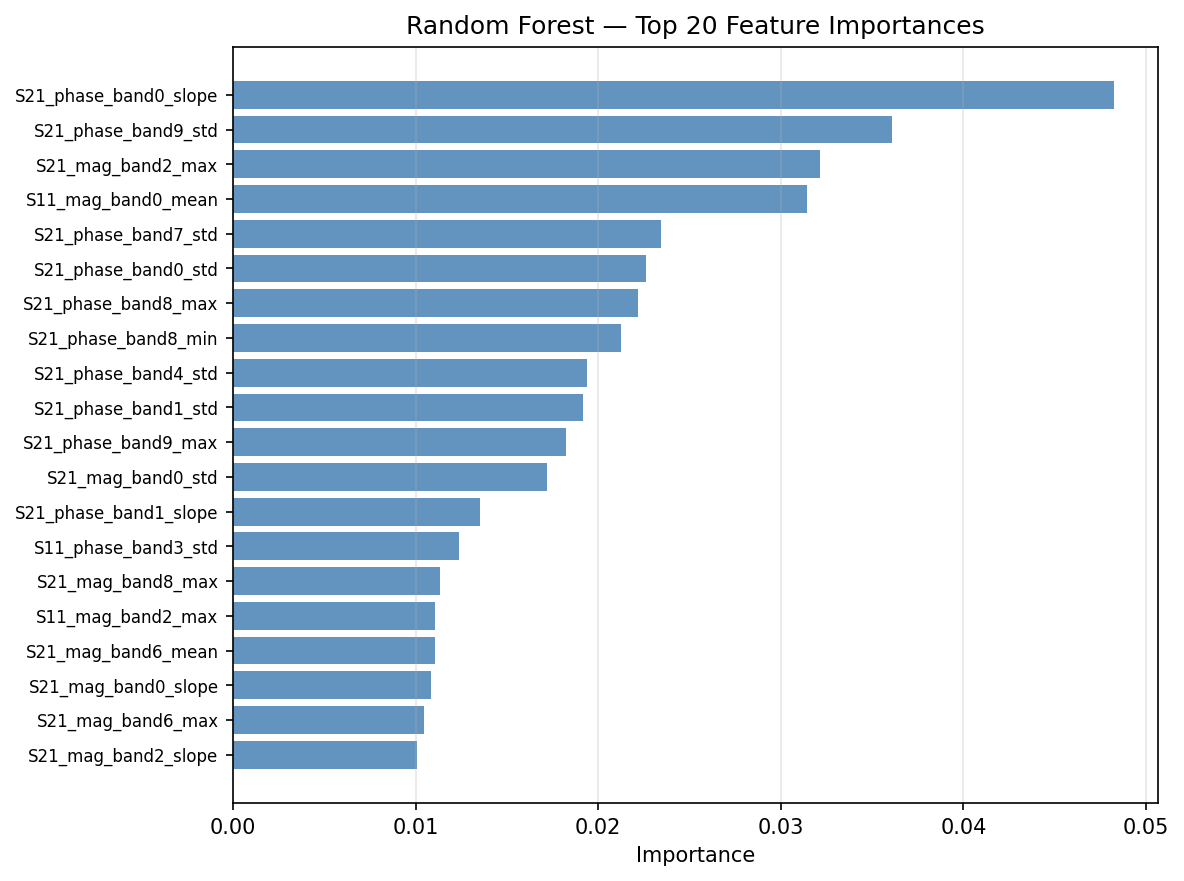
\includegraphics[width=0.85\textwidth]{rf_feature_importance}
  \caption{Top-20 Random Forest feature importances. $S_{21}$ phase features in the lowest three frequency bands (1.0--1.6\,GHz) dominate. Physically, $S_{21}$ phase encodes the dielectric propagation delay through tissue layers, and lower frequencies penetrate deeper into fat and muscle.}
  \label{fig:rf_importance}
\end{figure}

This result is physically interpretable: $S_{21}$ phase encodes the dielectric propagation delay accumulated as the wave travels through all tissue layers. Low frequencies (1.0--1.6\,GHz) penetrate the deepest, reaching both fat and muscle, and thus carry the most information about the tissue configuration of interest.

%=============================================================================
\chapter{Models}
\label{ch:models}
%=============================================================================

\section{Deterministic Baseline Models}

\subsection{Random Forest}

A Random Forest regressor~\cite{breiman2001} with 200 trees is trained directly on all three targets simultaneously (scikit-learn's \texttt{MultiOutputRegressor}-like internal handling). Band-statistical features (200-dimensional) are used; no feature scaling is needed since tree splits are invariant to monotone transforms. Feature importance is available via mean decrease in impurity.

\subsection{XGBoost}

XGBoost~\cite{chen2016} is wrapped in a \texttt{MultiOutputRegressor} for three-target prediction. Gradient-boosted trees are generally faster than Random Forests and handle feature interactions efficiently. Band-statistical features are used.

\subsection{Fully Connected Neural Network (FCNN)}

A three-hidden-layer FCNN (scikit-learn \texttt{MLPRegressor}) with architecture $800 \to 256 \to 128 \to 64 \to 3$, ReLU activations, and Adam optimiser is used as a neural baseline. This model uses scaled 800-dimensional features but produces only point estimates with no uncertainty.

\section{MC Dropout Neural Network}

\subsection{Architecture}

\begin{equation}
\begin{aligned}
  &\text{Encoder:} \quad \mathrm{Linear}(800\to 256) \to \mathrm{BN} \to \mathrm{ReLU} \to \mathrm{Dropout}(p{=}0.3) \\
  &\phantom{\text{Encoder:}} \quad \mathrm{Linear}(256\to 128) \to \mathrm{BN} \to \mathrm{ReLU} \to \mathrm{Dropout}(p{=}0.3) \\
  &\phantom{\text{Encoder:}} \quad \mathrm{Linear}(128\to 64) \to \mathrm{BN} \to \mathrm{ReLU} \to \mathrm{Dropout}(p{=}0.3) \\
  &\text{Heads ($\times$3):} \quad \mathrm{Linear}(64 \to 2) \to [\hat\mu_k,\; \widehat{\log\sigma^2_k}]
\end{aligned}
\end{equation}

The shared encoder extracts a 64-dimensional tissue representation; each of the three independent heads predicts the mean and log-variance for one tissue target. Total trainable parameters: 247,494.

\subsection{Training}

\begin{itemize}[noitemsep]
  \item \textbf{Loss:} Heteroscedastic Gaussian NLL (Equation~\ref{eq:nll_loss}).
  \item \textbf{Optimiser:} Adam, learning rate $10^{-3}$, weight decay $10^{-4}$.
  \item \textbf{Scheduler:} \texttt{ReduceLROnPlateau} (patience 10, factor 0.5).
  \item \textbf{Early stopping:} patience 20 epochs; training stopped at epoch 34.
  \item \textbf{Mini-batch size:} 32.
  \item \textbf{Data split:} Volunteers 1--14 as train (323 files); volunteers 15--18 as internal validation (108 files).
\end{itemize}

Figure~\ref{fig:mc_curves} shows the training and validation loss curves.

\begin{figure}[H]
  \centering
  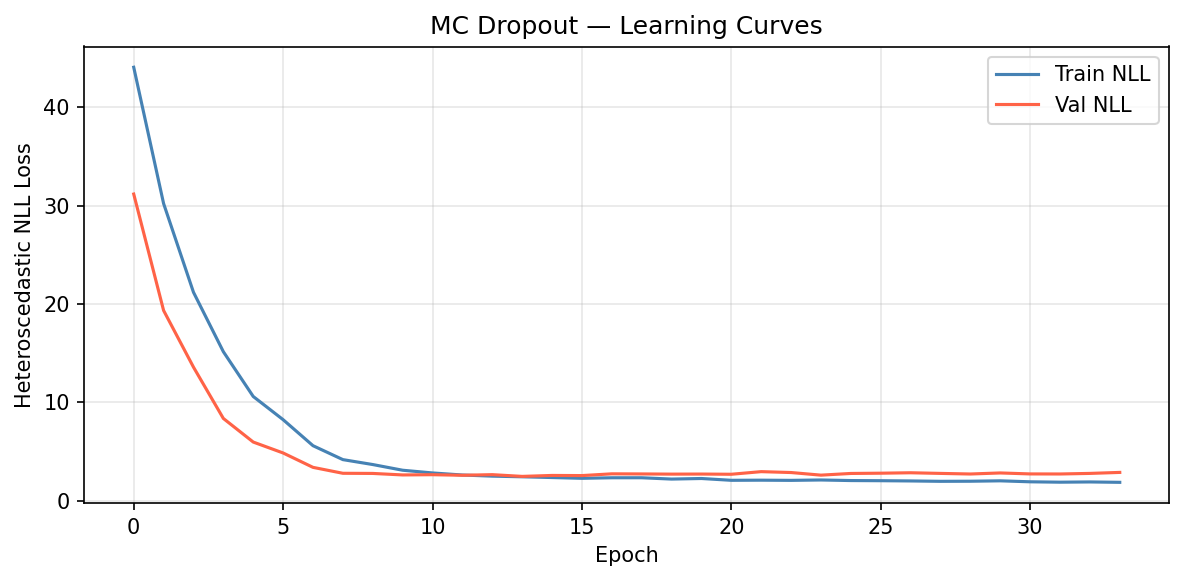
\includegraphics[width=0.92\textwidth]{mc_learning_curves}
  \caption{MC Dropout training and validation NLL loss curves. The model jointly learns to predict tissue thickness (mean) and calibrate its own uncertainty (variance) via the heteroscedastic Gaussian NLL objective. The marker indicates the best-validation epoch where early stopping would trigger.}
  \label{fig:mc_curves}
\end{figure}

\subsection{MC Inference}

At inference time, BatchNorm layers are set to eval mode (use running statistics) and Dropout layers are kept in \emph{train} mode. For each test sample, $T=50$ stochastic forward passes are performed, producing $\{\hat\mu_k^{(t)},\, \widehat{\log\sigma_k^{2(t)}}\}_{t=1}^{50}$. The epistemic and aleatoric uncertainty components are computed via Equations~\ref{eq:mc_mean}--\ref{eq:mc_ale}.

\section{Deep Ensembles}

\subsection{Architecture}

Each of the $M=5$ ensemble members uses the same encoder and head architecture as MC Dropout but \emph{without Dropout layers}. Stochasticity arises exclusively from independent random weight initialisations and mini-batch ordering. Each member is trained independently with a unique random seed (seed $=$ 42 $+$ member index).

\subsection{Training}

Training protocol identical to MC Dropout (Adam, ReduceLROnPlateau, early stopping, patience 20). Members converged in 27--32 epochs. Figure~\ref{fig:ens_curves} shows validation loss per member.

\begin{figure}[H]
  \centering
  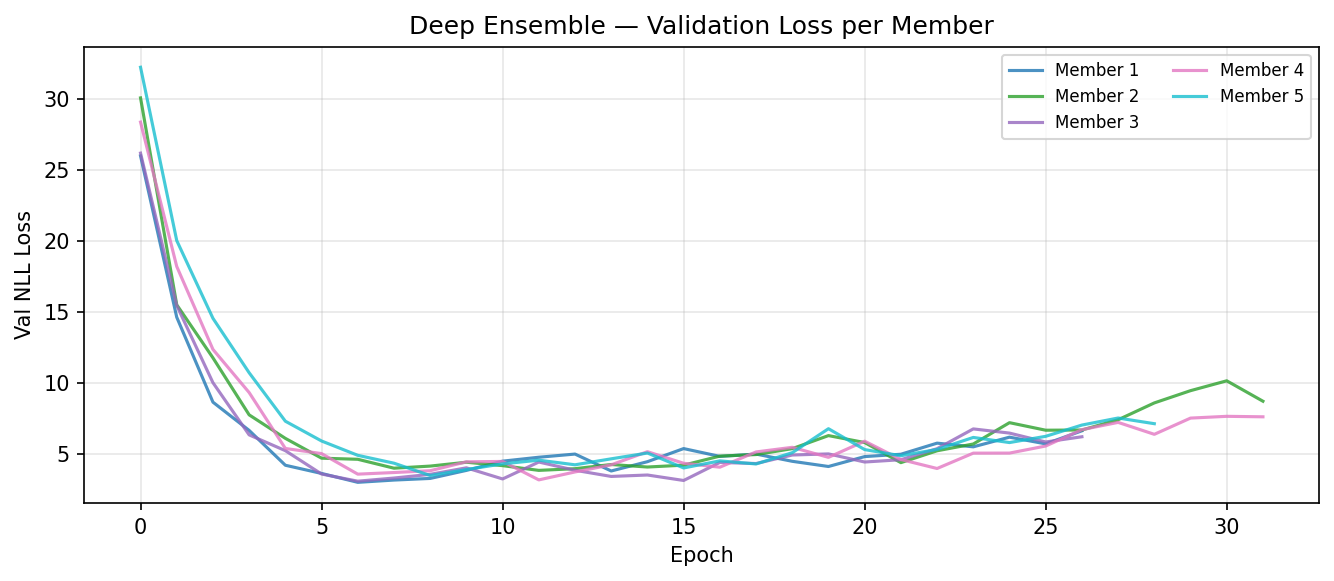
\includegraphics[width=0.92\textwidth]{ensemble_learning_curves}
  \caption{Deep Ensemble validation NLL loss curves for all five independently initialised members. Curves converge to similar final values while following different trajectories, confirming functional diversity across members---the prerequisite for meaningful epistemic uncertainty estimates.}
  \label{fig:ens_curves}
\end{figure}

\subsection{Ensemble Aggregation}

Ensemble predictions are aggregated via the mixture-of-Gaussians rule. The epistemic component is the variance of the member means; the aleatoric component is the mean of the member-predicted variances.

%=============================================================================
\chapter{Experiments and Results}
\label{ch:results}
%=============================================================================

\section{Experimental Setup}

All experiments run on a CPU workstation. The full pipeline is implemented in Python (PyTorch for neural networks, scikit-learn for baselines). Key configuration:

\begin{itemize}[noitemsep]
  \item September 2022: 431 training samples, 16 volunteers; 800-dim features (neural) / 200-dim band features (trees).
  \item Internal validation: volunteers 15--18, 108 samples (neural network training control only).
  \item Independent test: March 2023, 23 volunteers, 471 samples (final evaluation).
\end{itemize}

\section{Cross-Validated Baseline Results}

Table~\ref{tab:cv} reports cross-validated RMSE (mean $\pm$ std across 4 folds) for the three deterministic baselines on the September 2022 cohort.

\begin{table}[H]
  \centering
  \caption{GroupKFold 4-fold cross-validated baseline results (September 2022). RMSE mean $\pm$ std across 4 folds.}
  \label{tab:cv}
  \begin{tabular}{lccc}
    \toprule
    \textbf{Model} & \textbf{Skin RMSE (mm)} & \textbf{Fat RMSE (mm)} & \textbf{Muscle RMSE (cm$^2$)} \\
    \midrule
    Random Forest & $0.349 \pm 0.047$ & $5.703 \pm 0.513$ & $2.088 \pm 0.959$ \\
    XGBoost       & $0.343 \pm 0.042$ & $5.798 \pm 0.582$ & $2.222 \pm 1.002$ \\
    FCNN          & $0.428 \pm 0.028$ & $5.770 \pm 0.844$ & $2.218 \pm 1.010$ \\
    \bottomrule
  \end{tabular}
\end{table}

All three models show negative R$^2$ in the majority of folds. The interpretation of this finding is deferred to Section~\ref{sec:negative_r2}, where it is identified as the central empirical result of the thesis.

\section{MC Dropout: Internal Validation Results}

Tables~\ref{tab:mc_internal} and~\ref{tab:mc_unc} report performance and uncertainty decomposition on the September 2022 internal validation set (volunteers 15--18).

\begin{table}[H]
  \centering
  \caption{MC Dropout performance on September 2022 internal validation ($n=108$ samples).}
  \label{tab:mc_internal}
  \begin{tabular}{lcccccc}
    \toprule
    \textbf{Target} & \textbf{RMSE} & \textbf{MAE} & \textbf{R$^2$} & \textbf{PICP 95\%} & \textbf{ECE} & \textbf{NLL} \\
    \midrule
    Skin (mm)     & 0.700 & 0.632 & $-4.57$  & 0.861 & 0.208 & 1.191 \\
    Fat (mm)      & 5.059 & 5.046 & $-526.0$ & 1.000 & 0.204 & 3.298 \\
    Muscle (cm$^2$) & 1.354 & 1.106 & $-0.23$  & 1.000 & 0.112 & 1.845 \\
    \bottomrule
  \end{tabular}
\end{table}

\begin{table}[H]
  \centering
  \caption{MC Dropout uncertainty decomposition, internal validation.}
  \label{tab:mc_unc}
  \begin{tabular}{lcc}
    \toprule
    \textbf{Target} & \textbf{Epistemic $\sigma$ (mean)} & \textbf{Aleatoric $\sigma$ (mean)} \\
    \midrule
    Skin (mm)       & 0.259 mm   & 0.446 mm   \\
    Fat (mm)        & 0.700 mm   & 9.281 mm   \\
    Muscle (cm$^2$) & 0.618 cm$^2$ & 1.937 cm$^2$ \\
    \bottomrule
  \end{tabular}
\end{table}

Figures~\ref{fig:mc_unc_skin}--\ref{fig:mc_unc_muscle} show the uncertainty distribution plots for the internal validation set. Each three-panel figure displays (left) predicted mean vs.\ ground truth with $\pm 2\sigma$ error bars, (centre) epistemic vs.\ aleatoric decomposition per sample, and (right) histogram of total predictive standard deviation.

\begin{figure}[H]
  \centering
  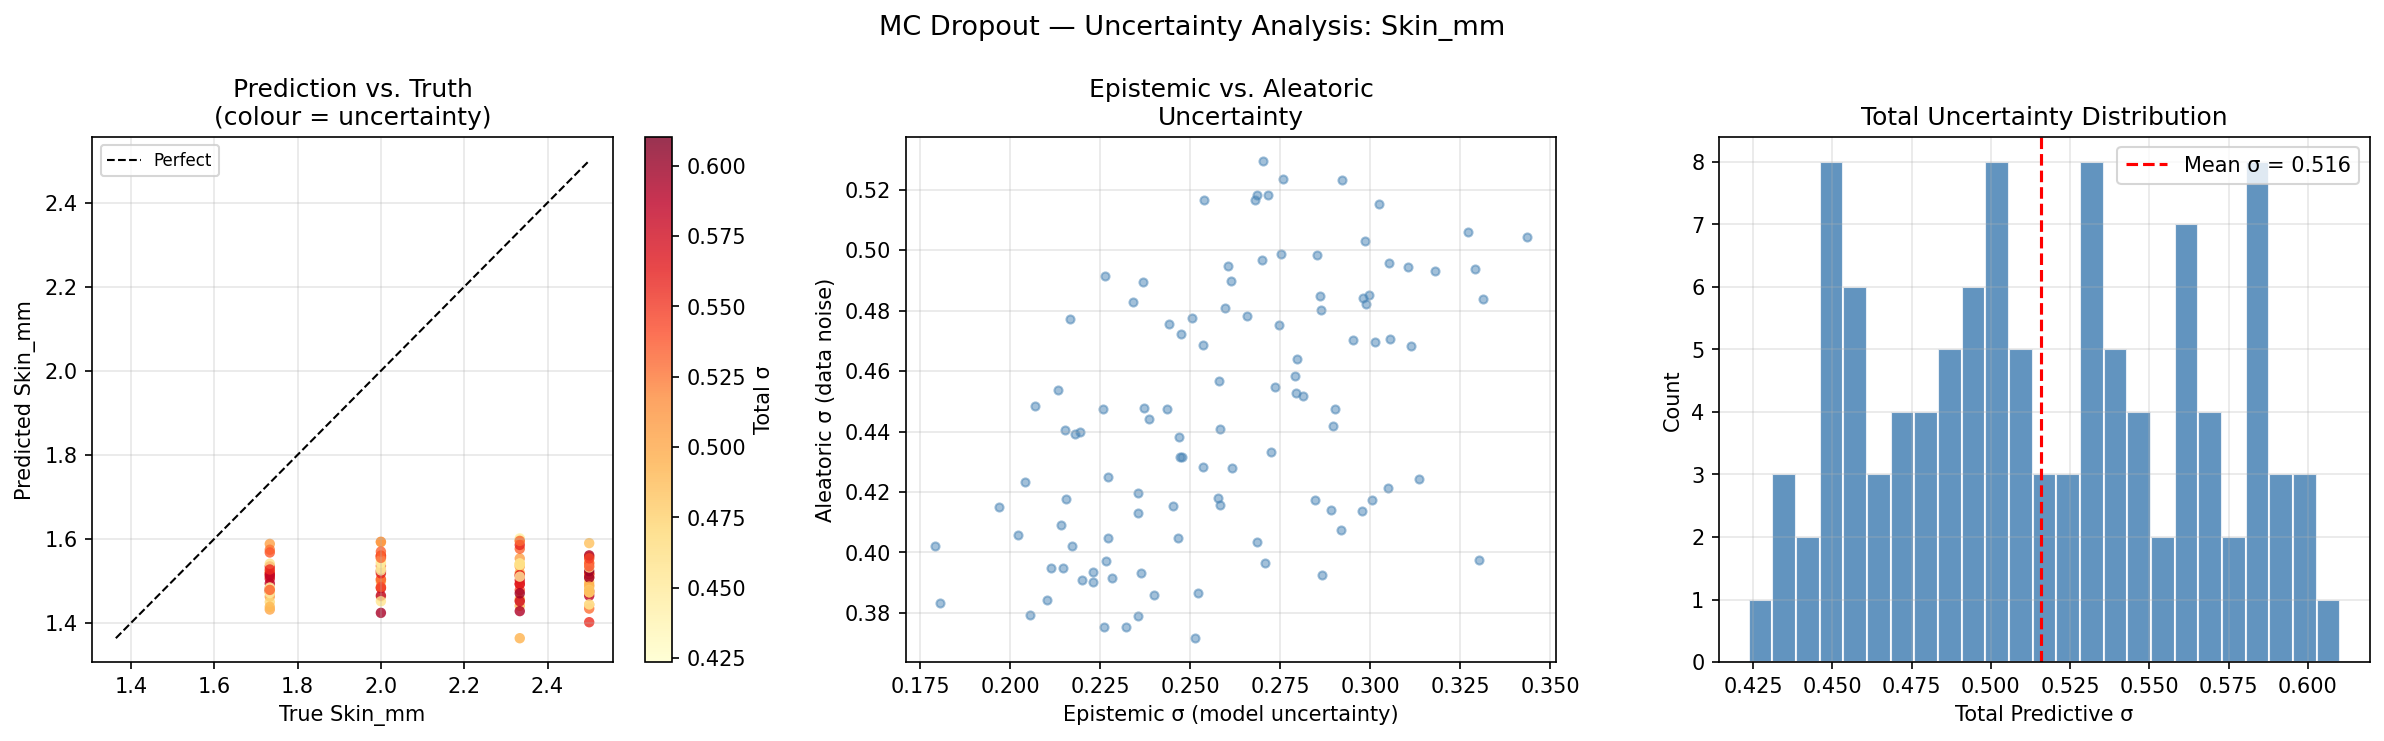
\includegraphics[width=\textwidth]{mc_uncertainty_skin}
  \caption{MC Dropout uncertainty analysis for Skin thickness (internal validation). Left: predicted mean $\pm 2\sigma_{\mathrm{total}}$ vs.\ ground truth. Centre: epistemic vs.\ aleatoric uncertainty per sample. Right: distribution of $\sigma_{\mathrm{total}}$.}
  \label{fig:mc_unc_skin}
\end{figure}

\begin{figure}[H]
  \centering
  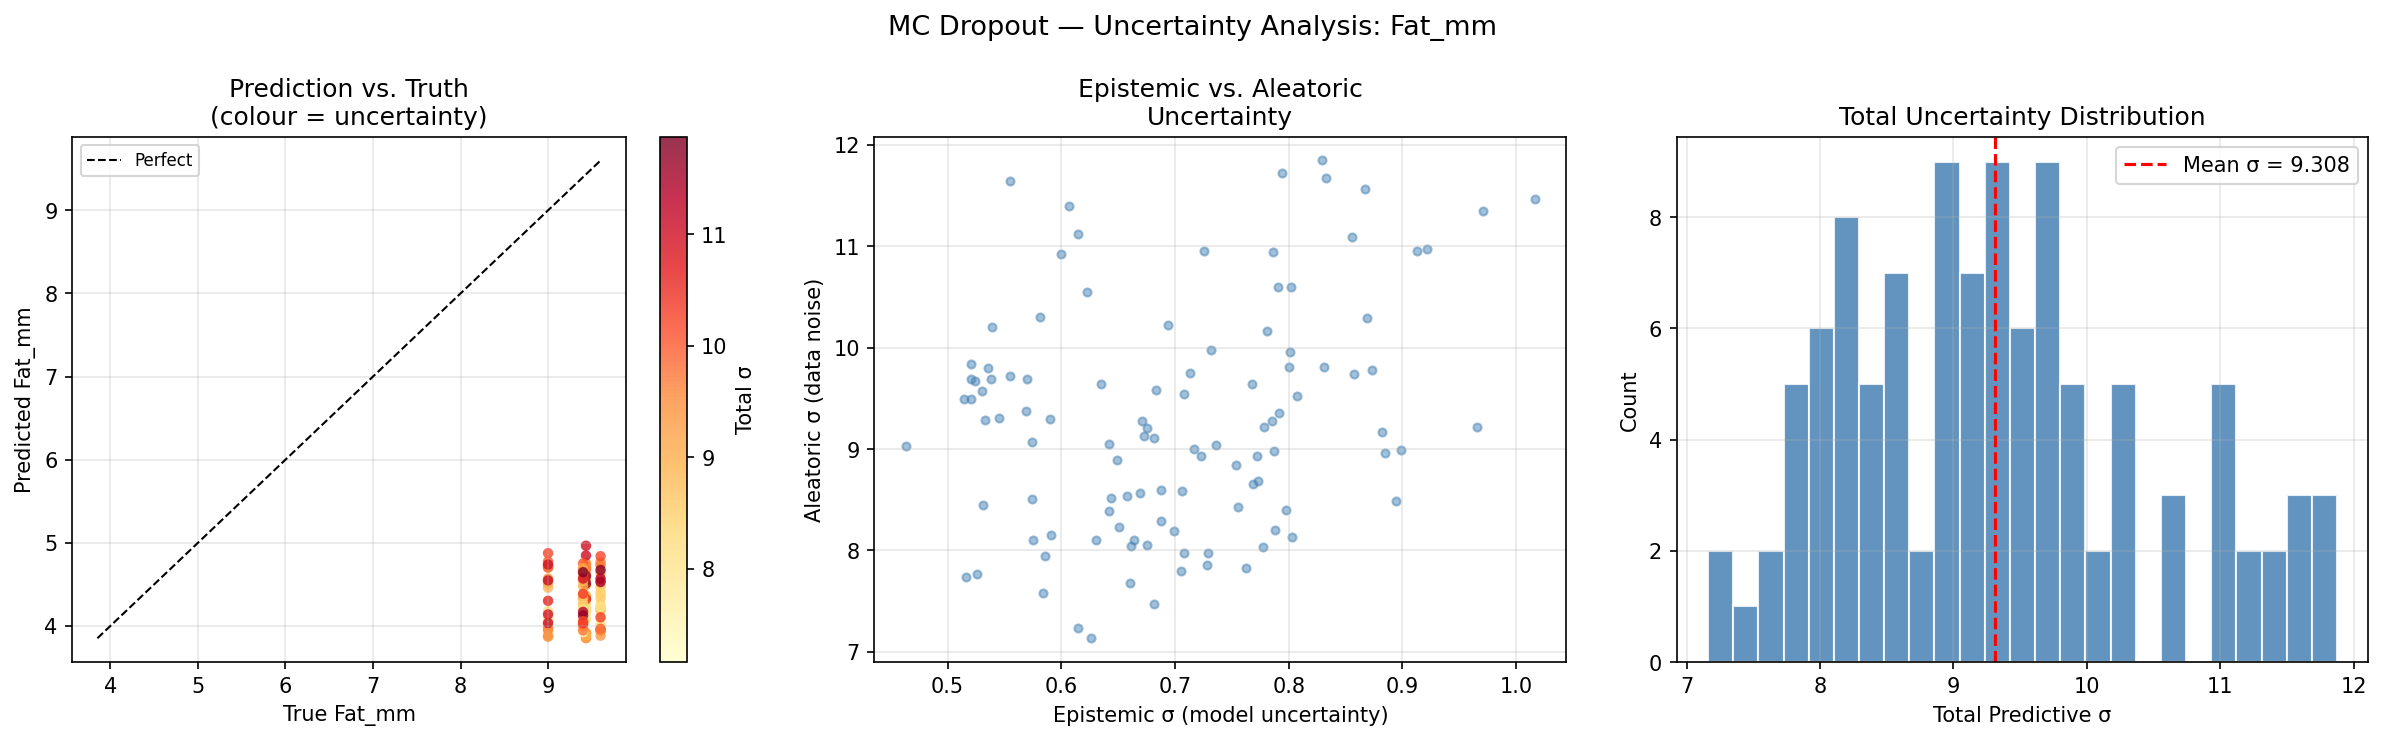
\includegraphics[width=\textwidth]{mc_uncertainty_fat}
  \caption{MC Dropout uncertainty analysis for Fat thickness (internal validation). The aleatoric uncertainty ($\bar\sigma_{\mathrm{ale}}=9.28$\,mm) dominates, indicating that the microwave-to-fat mapping carries high irreducible noise at this dataset size.}
  \label{fig:mc_unc_fat}
\end{figure}

\begin{figure}[H]
  \centering
  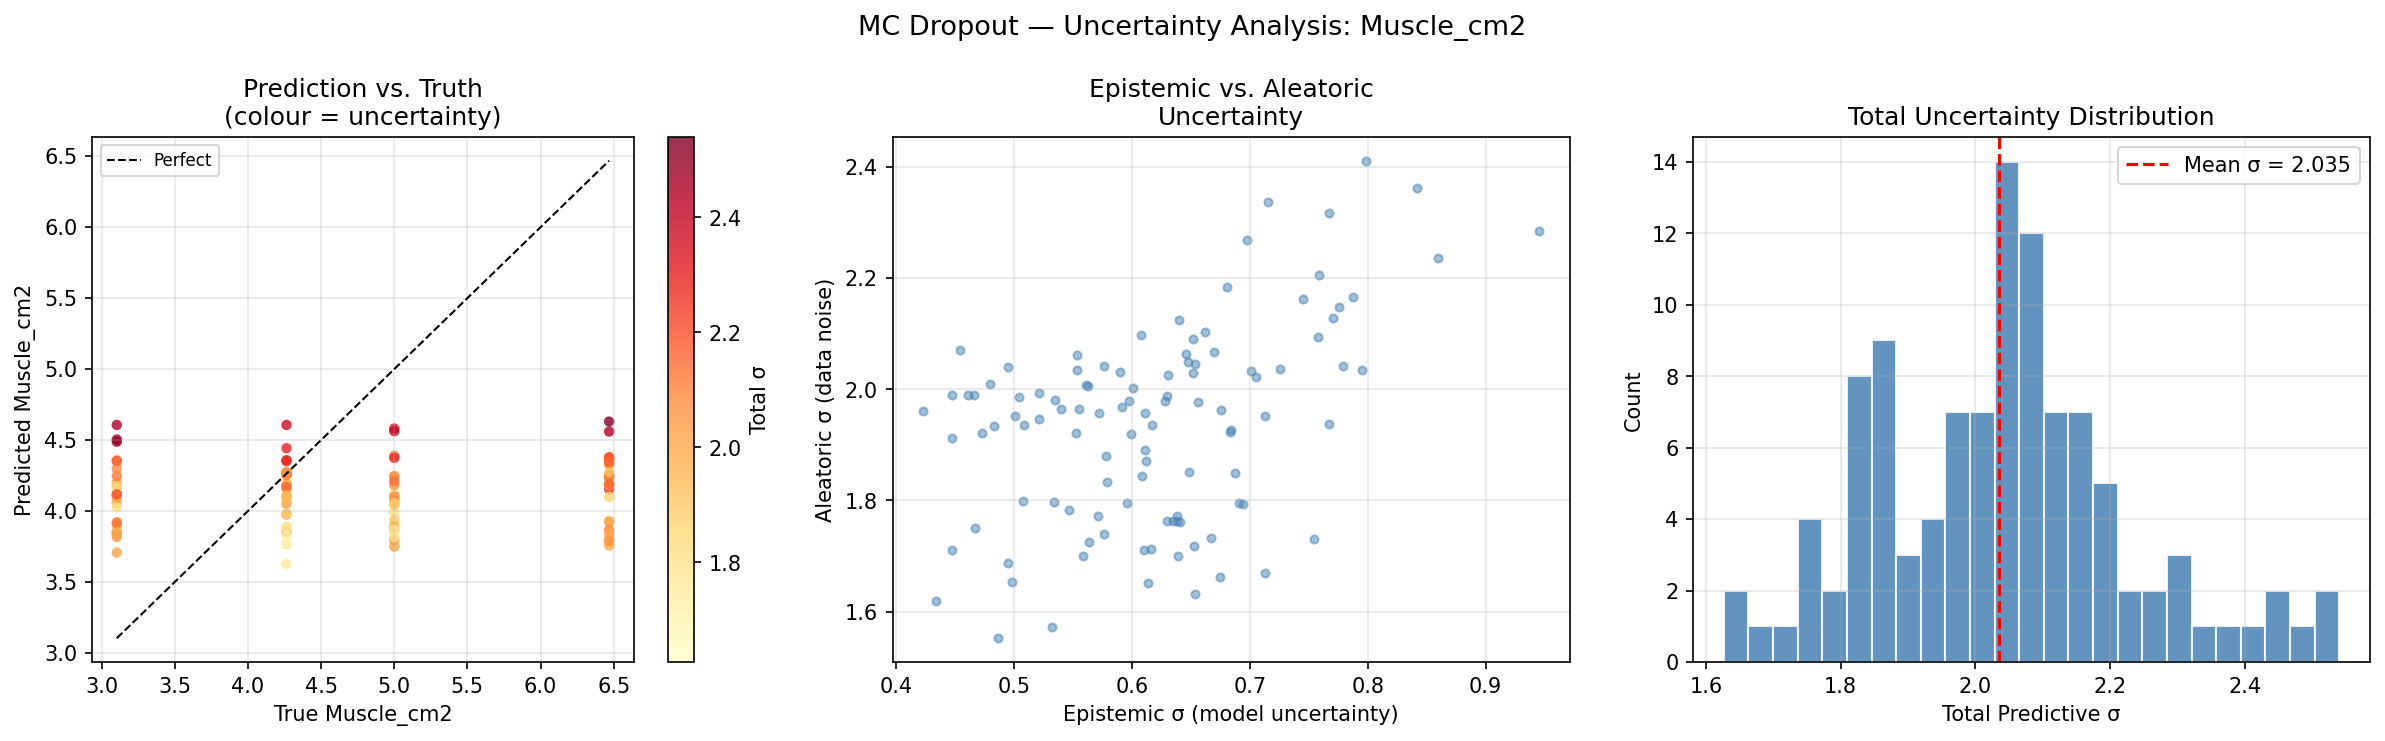
\includegraphics[width=\textwidth]{mc_uncertainty_muscle}
  \caption{MC Dropout uncertainty analysis for Muscle CSA (internal validation). Both epistemic and aleatoric components are meaningful; the model shows the best calibration for this target (ECE\,=\,0.112).}
  \label{fig:mc_unc_muscle}
\end{figure}

\section{Deep Ensemble: Internal Validation Results}

Tables~\ref{tab:ens_internal} and~\ref{tab:ens_unc} report Deep Ensemble results on the same internal validation partition.

\begin{table}[H]
  \centering
  \caption{Deep Ensemble performance on September 2022 internal validation ($n=108$ samples).}
  \label{tab:ens_internal}
  \begin{tabular}{lcccccc}
    \toprule
    \textbf{Target} & \textbf{RMSE} & \textbf{MAE} & \textbf{R$^2$} & \textbf{PICP 95\%} & \textbf{ECE} & \textbf{NLL} \\
    \midrule
    Skin (mm)       & 0.704 & 0.632 & $-4.63$  & 0.787 & 0.217 & 1.246 \\
    Fat (mm)        & 6.408 & 6.404 & $-845.0$ & 1.000 & 0.302 & 3.393 \\
    Muscle (cm$^2$) & 1.967 & 1.605 & $-1.60$  & 1.000 & 0.037 & 2.117 \\
    \bottomrule
  \end{tabular}
\end{table}

\begin{table}[H]
  \centering
  \caption{Deep Ensemble uncertainty decomposition, internal validation.}
  \label{tab:ens_unc}
  \begin{tabular}{lcc}
    \toprule
    \textbf{Target} & \textbf{Epistemic $\sigma$ (mean)} & \textbf{Aleatoric $\sigma$ (mean)} \\
    \midrule
    Skin (mm)       & 0.167 mm   & 0.426 mm   \\
    Fat (mm)        & 0.822 mm   & 4.849 mm   \\
    Muscle (cm$^2$) & 0.643 cm$^2$ & 2.116 cm$^2$ \\
    \bottomrule
  \end{tabular}
\end{table}

Figures~\ref{fig:ens_unc_skin}--\ref{fig:ens_unc_muscle} show the ensemble uncertainty distributions for internal validation.

\begin{figure}[H]
  \centering
  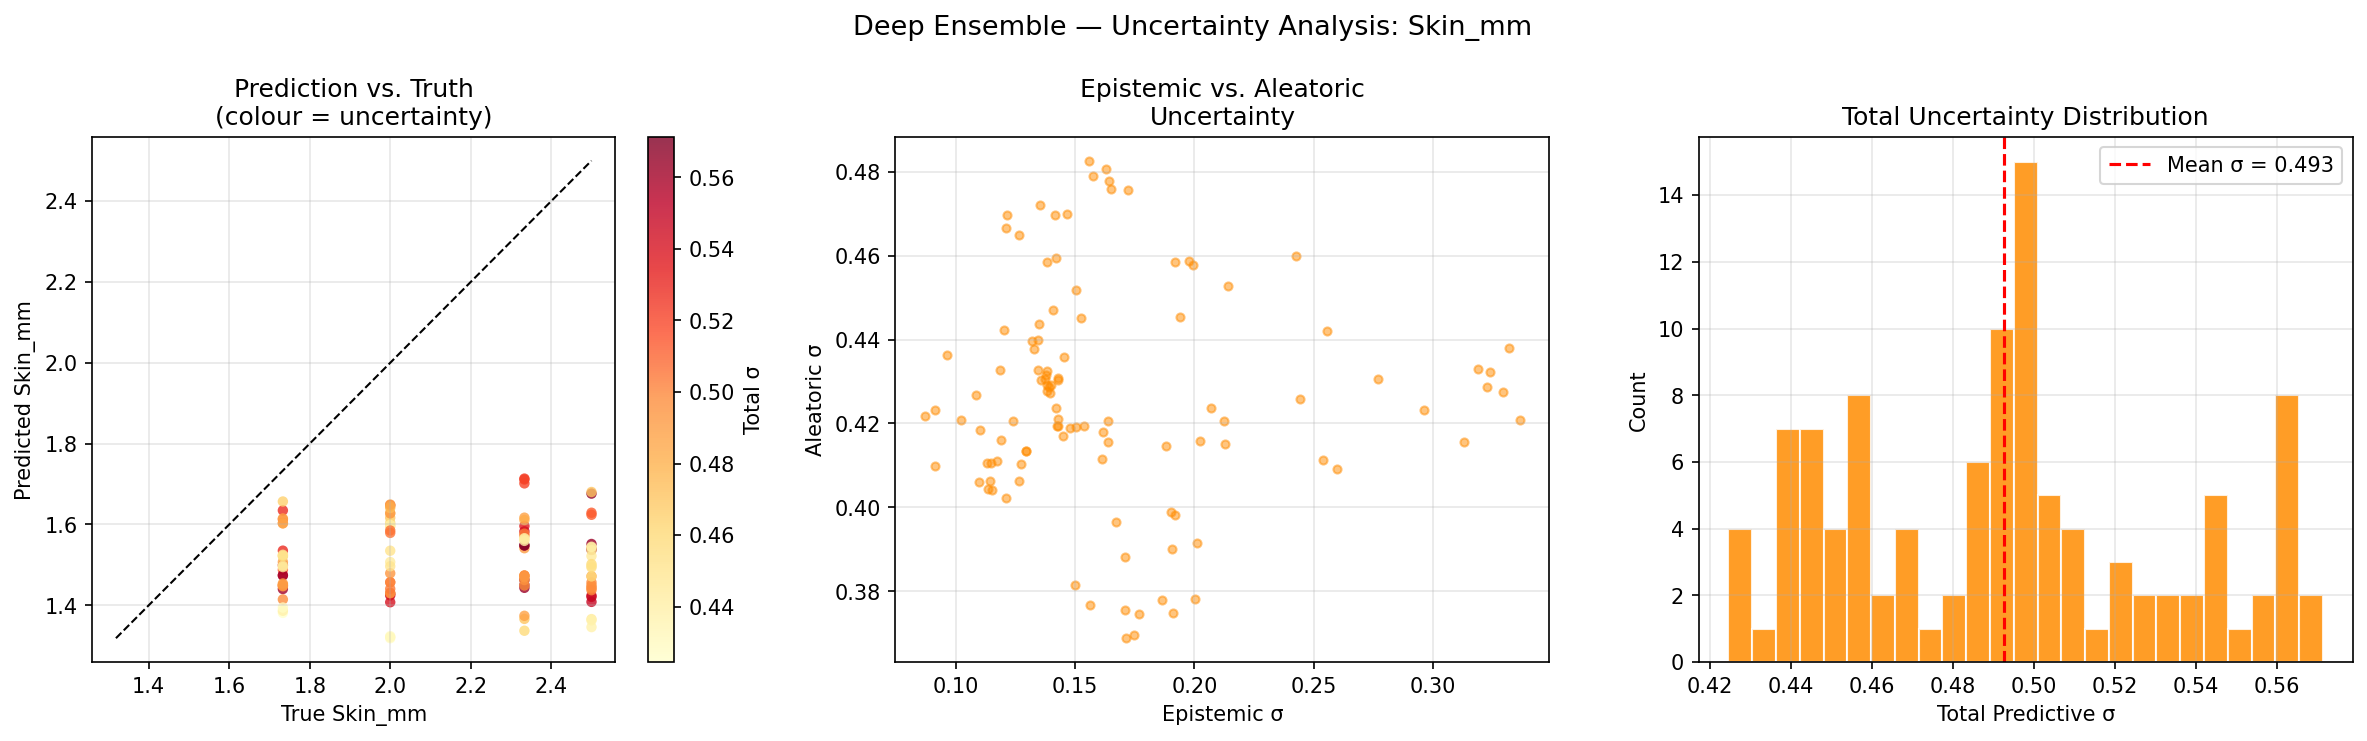
\includegraphics[width=\textwidth]{ens_uncertainty_skin}
  \caption{Deep Ensemble uncertainty analysis for Skin thickness (internal validation).}
  \label{fig:ens_unc_skin}
\end{figure}

\begin{figure}[H]
  \centering
  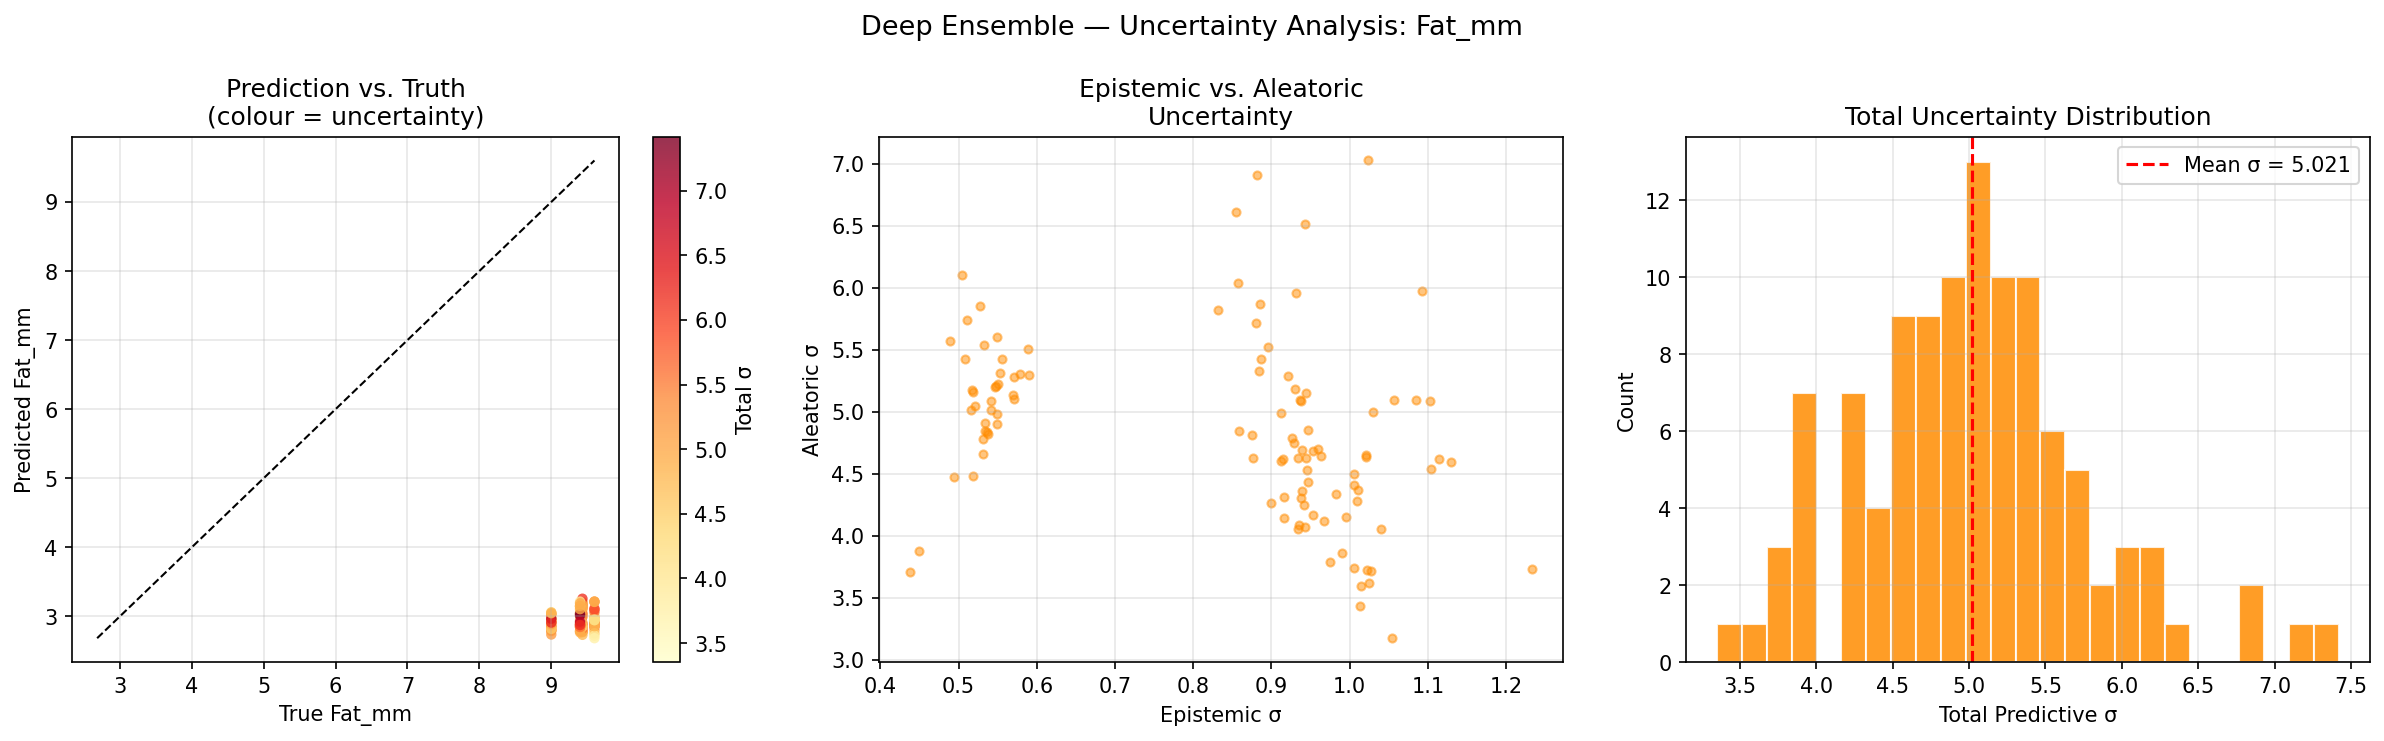
\includegraphics[width=\textwidth]{ens_uncertainty_fat}
  \caption{Deep Ensemble uncertainty analysis for Fat thickness (internal validation). The Deep Ensemble aleatoric fat uncertainty ($\bar\sigma_{\mathrm{ale}}=4.85$\,mm) is lower than MC Dropout's (9.28\,mm) but the RMSE is higher (6.41 vs.\ 5.06\,mm), indicating different calibration failure modes.}
  \label{fig:ens_unc_fat}
\end{figure}

\begin{figure}[H]
  \centering
  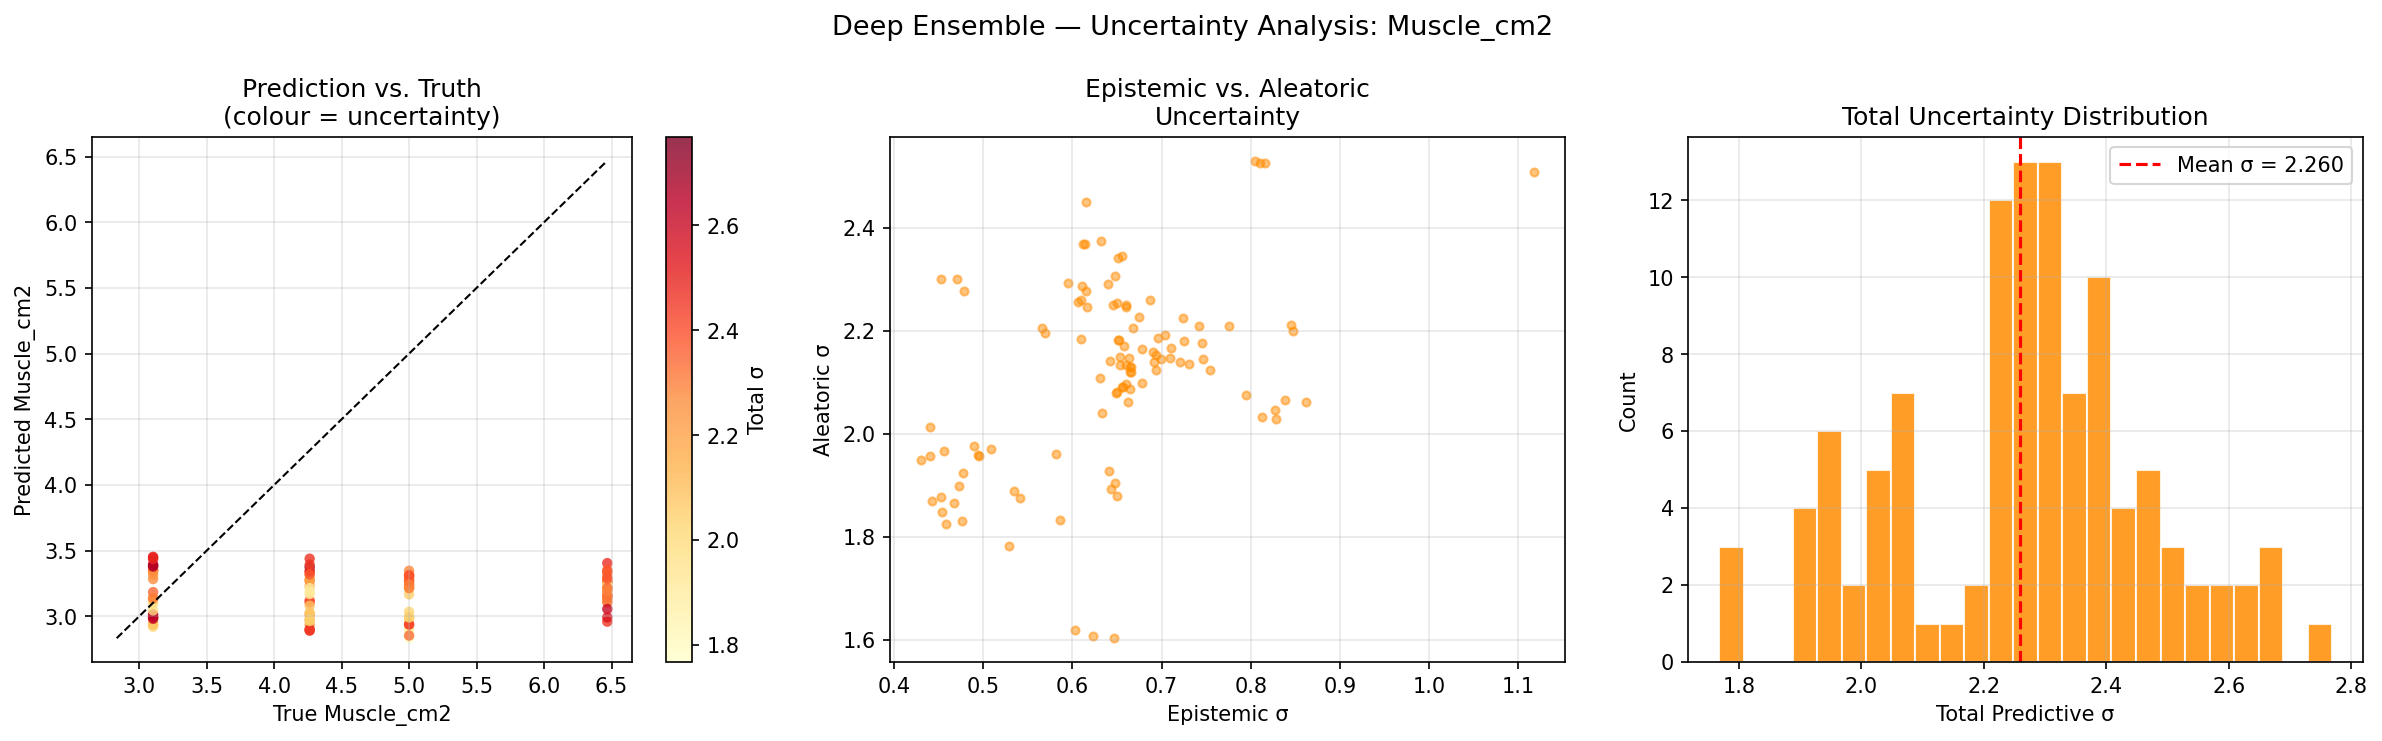
\includegraphics[width=\textwidth]{ens_uncertainty_muscle}
  \caption{Deep Ensemble uncertainty analysis for Muscle CSA (internal validation). The ECE of 0.037 is the best calibration result across all model--target combinations on the internal validation set.}
  \label{fig:ens_unc_muscle}
\end{figure}

\section{Independent Validation: March 2023 (Definitive Results)}

The following tables present the final evaluation on the March 2023 independent test set.

\begin{table}[H]
  \centering
  \caption{RMSE and R$^2$ on the March 2023 independent test set ($n=471$, 23 volunteers).}
  \label{tab:val_rmse}
  \begin{tabular}{lcccccc}
    \toprule
    \multirow{2}{*}{\textbf{Model}} &
    \multicolumn{2}{c}{\textbf{Skin (mm)}} &
    \multicolumn{2}{c}{\textbf{Fat (mm)}} &
    \multicolumn{2}{c}{\textbf{Muscle (cm$^2$)}} \\
    \cmidrule(lr){2-3}\cmidrule(lr){4-5}\cmidrule(lr){6-7}
    & RMSE & R$^2$ & RMSE & R$^2$ & RMSE & R$^2$ \\
    \midrule
    Random Forest  & 0.422 & $-0.420$ & \textbf{4.473} & $-0.865$ & \textbf{2.111} & $-0.055$ \\
    XGBoost        & \textbf{0.382} & $-0.161$ & 4.641 & $-1.008$ & 2.173 & $-0.117$ \\
    FCNN           & 0.700 & $-2.903$ & 5.682 & $-2.010$ & 2.687 & $-0.709$ \\
    MC Dropout     & 0.585 & $-1.729$ & 5.700 & $-2.029$ & 2.202 & $-0.148$ \\
    Deep Ensemble  & 0.688 & $-2.771$ & 6.769 & $-3.271$ & 2.843 & $-0.913$ \\
    \bottomrule
  \end{tabular}
\end{table}

\begin{table}[H]
  \centering
  \caption{Calibration and probabilistic metrics on March 2023. ``---'' indicates the model produces no uncertainty output (PICP = 0, NLL $\to \infty$).}
  \label{tab:val_calib}
  \begin{tabular}{llccccc}
    \toprule
    \textbf{Metric} & \textbf{Target} & \textbf{RF} & \textbf{XGB} & \textbf{FCNN} & \textbf{MC Drop.} & \textbf{Ensemble} \\
    \midrule
    \multirow{3}{*}{ECE}
      & Skin     & --- & --- & --- & \textbf{0.074} & 0.110 \\
      & Fat      & --- & --- & --- & \textbf{0.094} & 0.199 \\
      & Muscle   & --- & --- & --- & \textbf{0.020} & 0.080 \\
    \midrule
    \multirow{3}{*}{PICP 95\%}
      & Skin     & 0.000 & 0.000 & 0.000 & 0.854 & \textbf{0.881} \\
      & Fat      & 0.000 & 0.000 & 0.000 & \textbf{1.000} & 0.786 \\
      & Muscle   & 0.000 & 0.000 & 0.000 & \textbf{0.926} & 0.871 \\
    \midrule
    \multirow{3}{*}{NLL}
      & Skin     & 89{,}133 & 72{,}911 & 245{,}054 & \textbf{0.930} & 1.108 \\
      & Fat      & $>$10\,M & $>$10\,M & $>$16\,M  & \textbf{3.310} & 3.679 \\
      & Muscle   & $>$2.2\,M & $>$2.4\,M & $>$3.6\,M & \textbf{2.250} & 2.617 \\
    \bottomrule
  \end{tabular}
\end{table}

Figures~\ref{fig:val_rf_skin}--\ref{fig:val_xgb_muscle} show prediction scatter plots for the tree-based baselines on the March 2023 test set.

\begin{figure}[H]
  \centering
  \begin{subfigure}[b]{0.47\textwidth}
    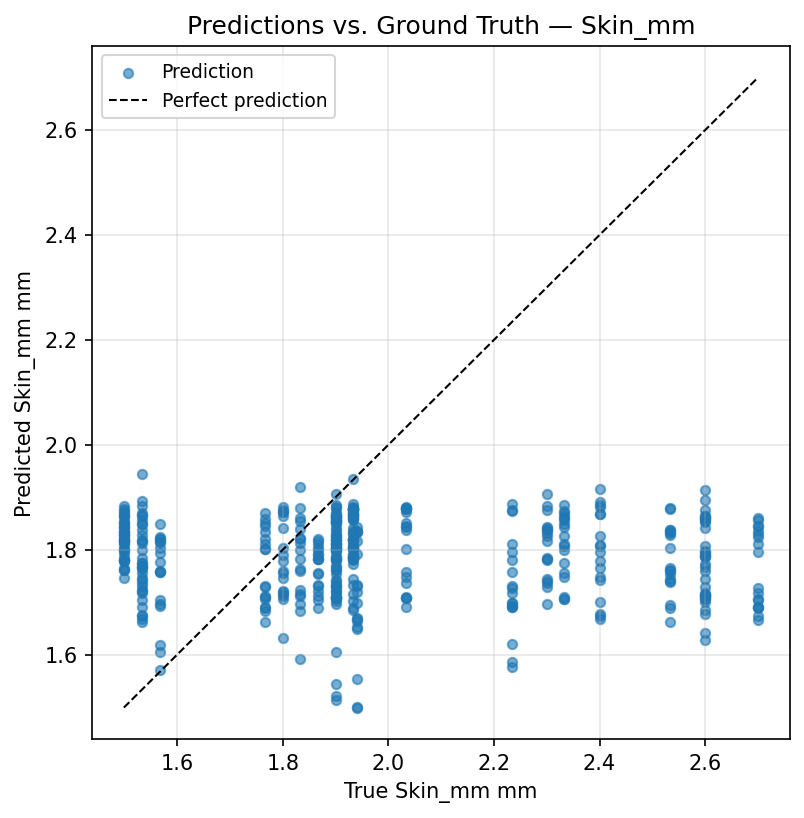
\includegraphics[width=\textwidth]{val_rf_skin}
    \caption{RF --- Skin thickness (mm)}
  \end{subfigure}\hfill
  \begin{subfigure}[b]{0.47\textwidth}
    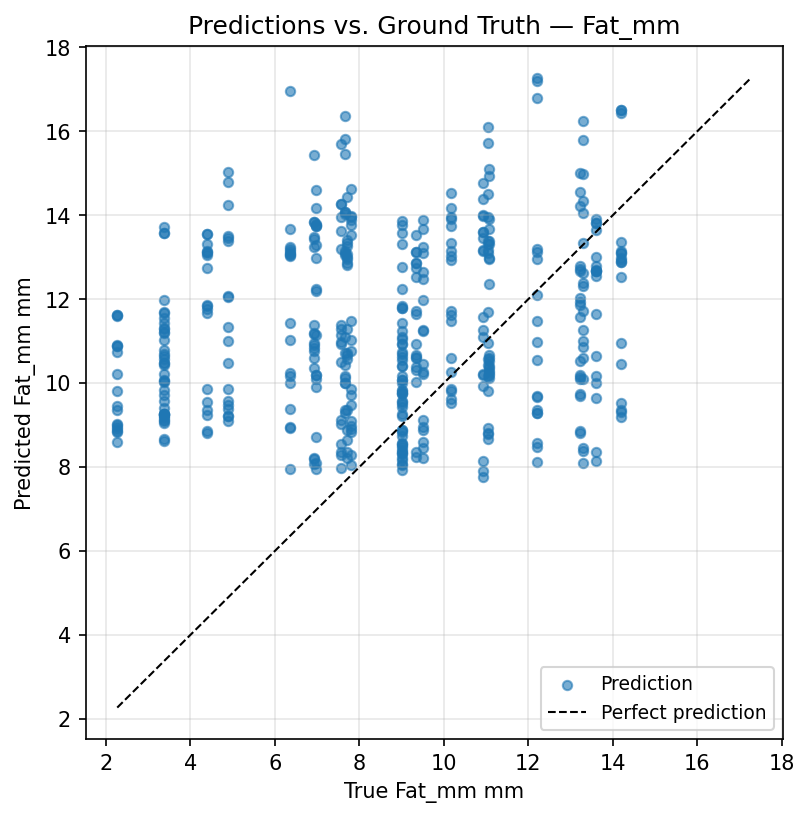
\includegraphics[width=\textwidth]{val_rf_fat}
    \caption{RF --- Subcutaneous fat thickness (mm)}
  \end{subfigure}

  \vspace{0.8em}
  \begin{subfigure}[b]{0.47\textwidth}
    \centering
    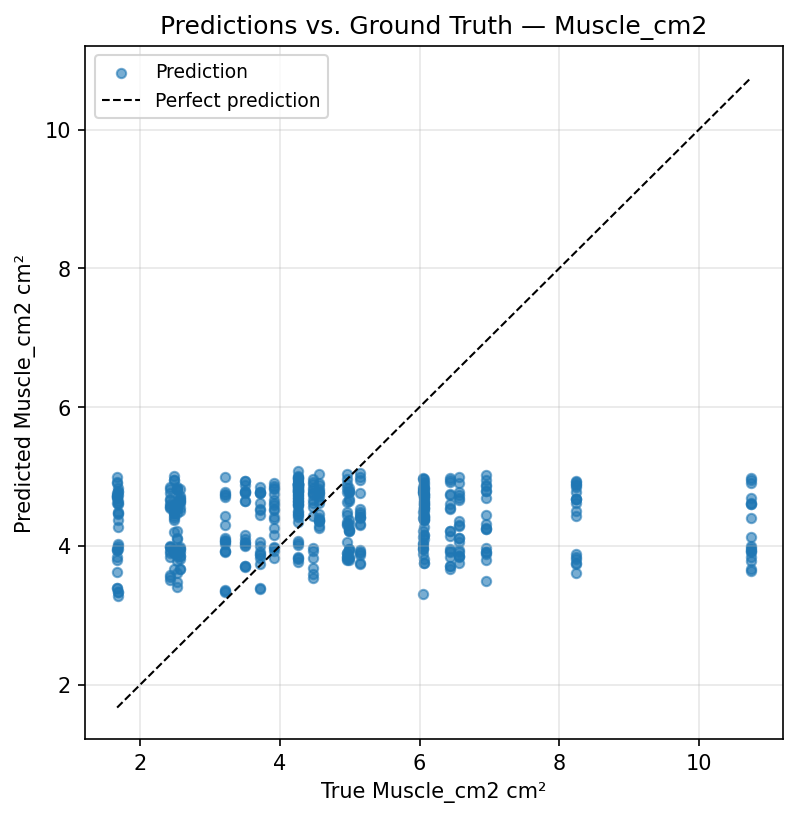
\includegraphics[width=\textwidth]{val_rf_muscle}
    \caption{RF --- Rectus femoris CSA (cm$^2$)}
  \end{subfigure}
  \caption{Random Forest predictions vs.\ ground truth on the March 2023 independent test set ($n=471$, 23 unseen volunteers). Each point is one test sample; the dashed diagonal represents perfect prediction. RMSE and MAE are annotated on each panel. No uncertainty bands are available for deterministic models.}
  \label{fig:val_rf_skin}
\end{figure}

\begin{figure}[H]
  \centering
  \begin{subfigure}[b]{0.47\textwidth}
    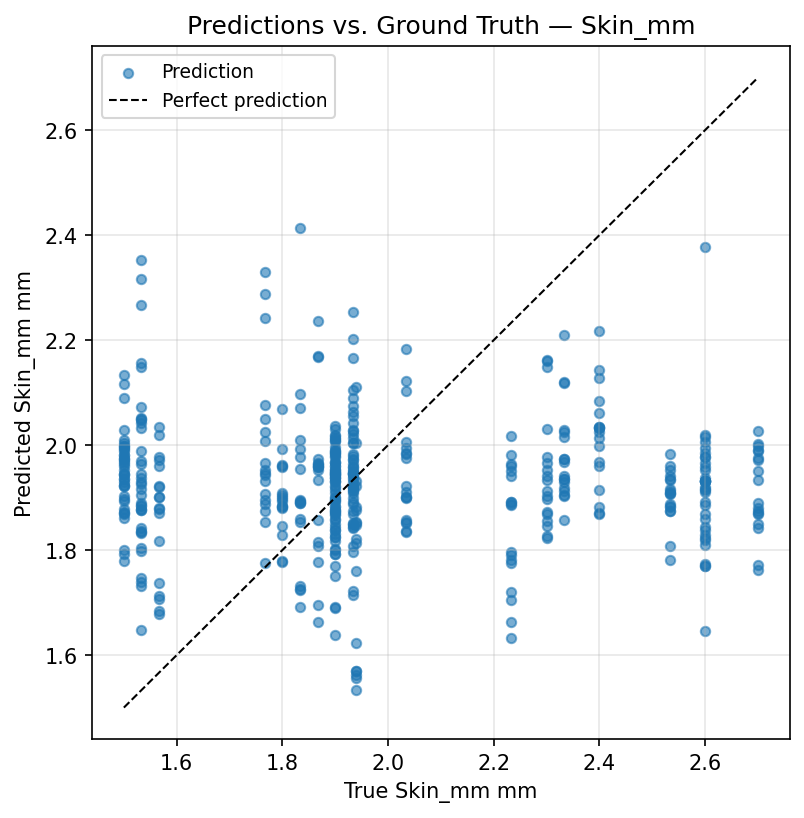
\includegraphics[width=\textwidth]{val_xgb_skin}
    \caption{XGBoost --- Skin thickness (mm)}
  \end{subfigure}\hfill
  \begin{subfigure}[b]{0.47\textwidth}
    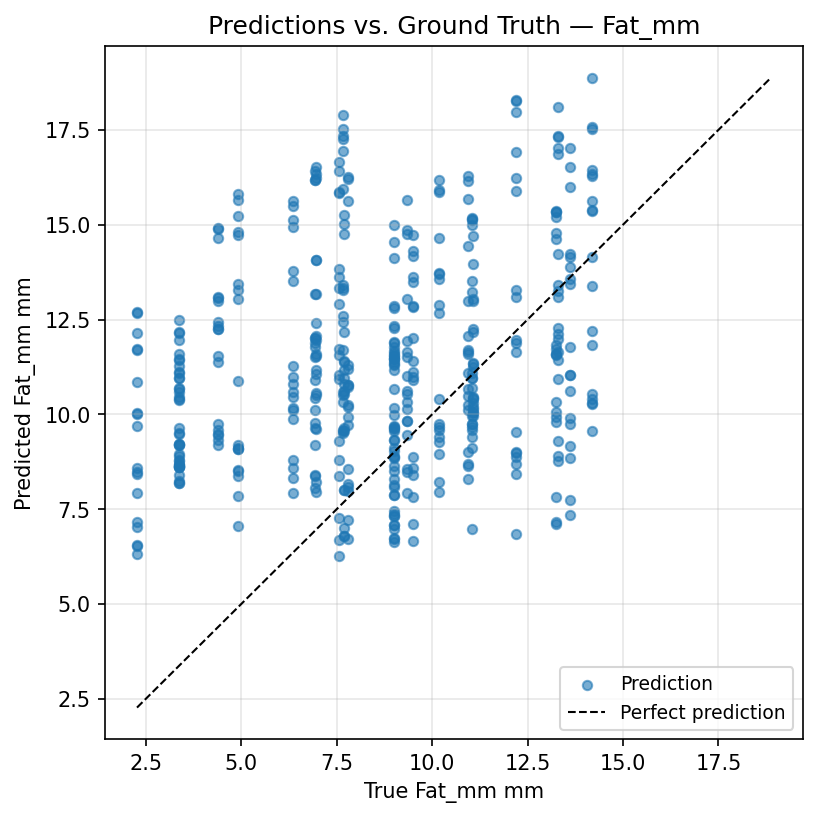
\includegraphics[width=\textwidth]{val_xgb_fat}
    \caption{XGBoost --- Subcutaneous fat thickness (mm)}
  \end{subfigure}

  \vspace{0.8em}
  \begin{subfigure}[b]{0.47\textwidth}
    \centering
    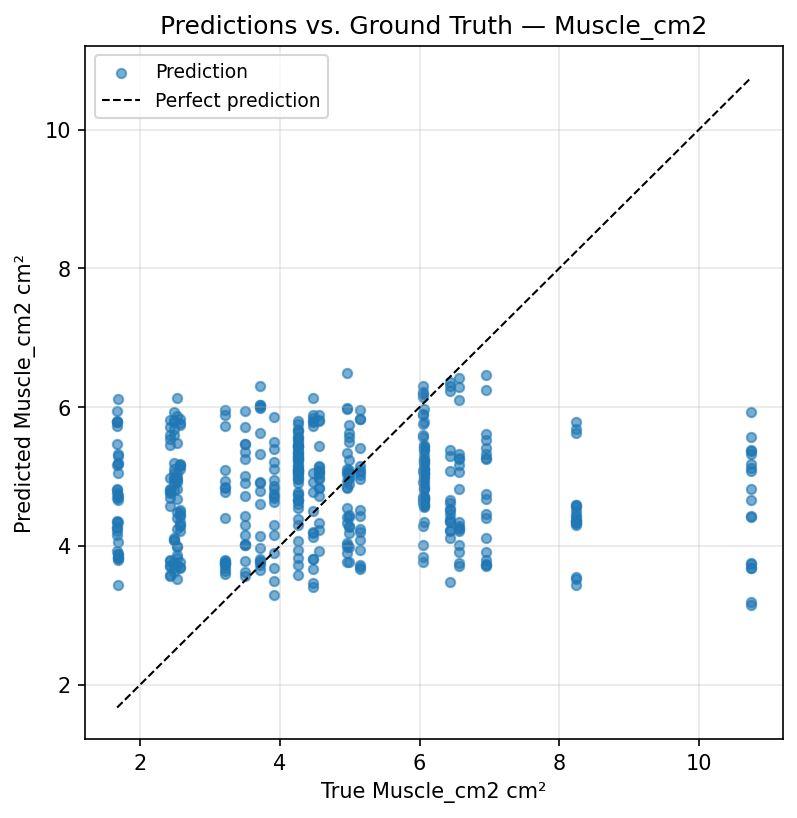
\includegraphics[width=\textwidth]{val_xgb_muscle}
    \caption{XGBoost --- Rectus femoris CSA (cm$^2$)}
  \end{subfigure}
  \caption{XGBoost predictions vs.\ ground truth on the March 2023 independent test set. XGBoost achieves the lowest RMSE for Skin (0.382\,mm) among all models, reflecting that tree-based methods have lower variance at small training cohort sizes.}
  \label{fig:val_xgb_muscle}
\end{figure}

Figures~\ref{fig:val_mc_skin}--\ref{fig:val_mc_muscle} show MC Dropout predictions with $\pm 2\sigma_{\mathrm{total}}$ error bars on the March 2023 test set.

\begin{figure}[H]
  \centering
  \begin{subfigure}[b]{0.47\textwidth}
    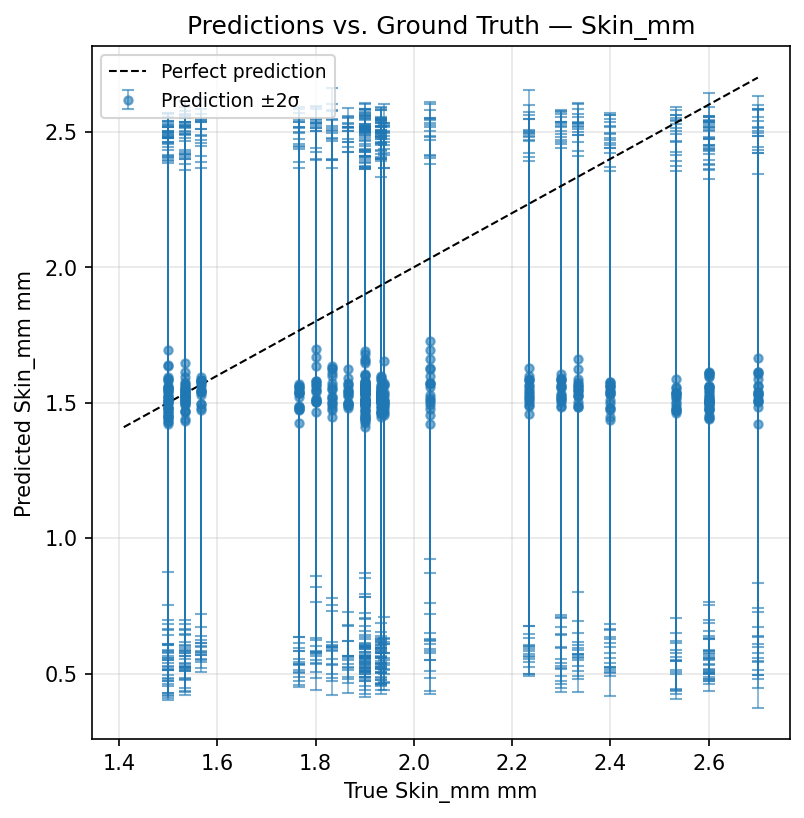
\includegraphics[width=\textwidth]{val_mc_skin}
    \caption{MC Dropout --- Skin thickness (mm)}
  \end{subfigure}\hfill
  \begin{subfigure}[b]{0.47\textwidth}
    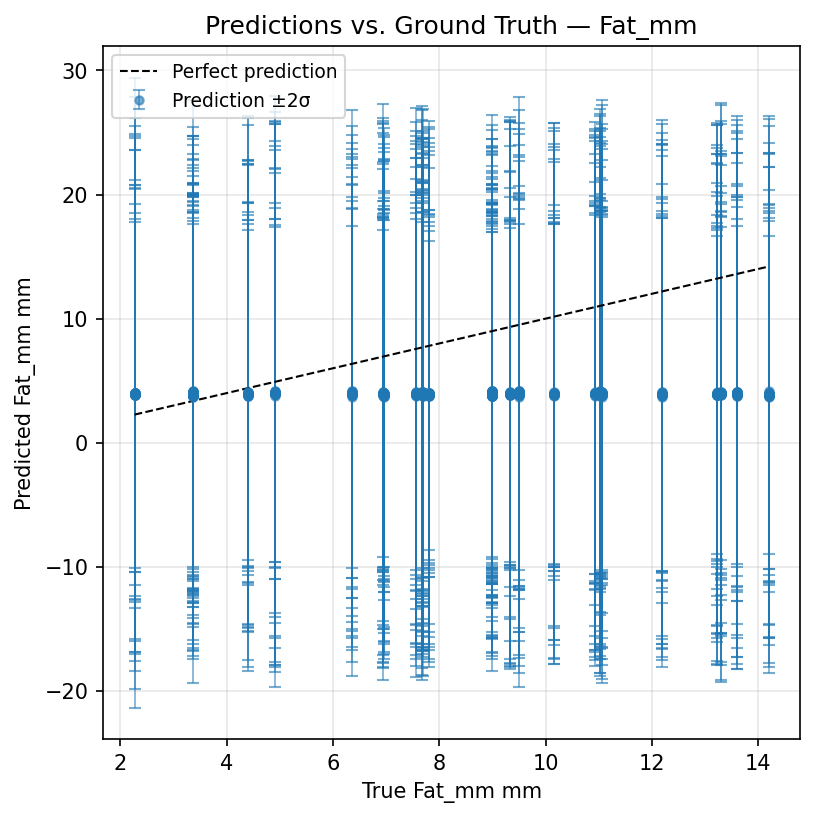
\includegraphics[width=\textwidth]{val_mc_fat}
    \caption{MC Dropout --- Subcutaneous fat thickness (mm)}
  \end{subfigure}

  \vspace{0.8em}
  \begin{subfigure}[b]{0.47\textwidth}
    \centering
    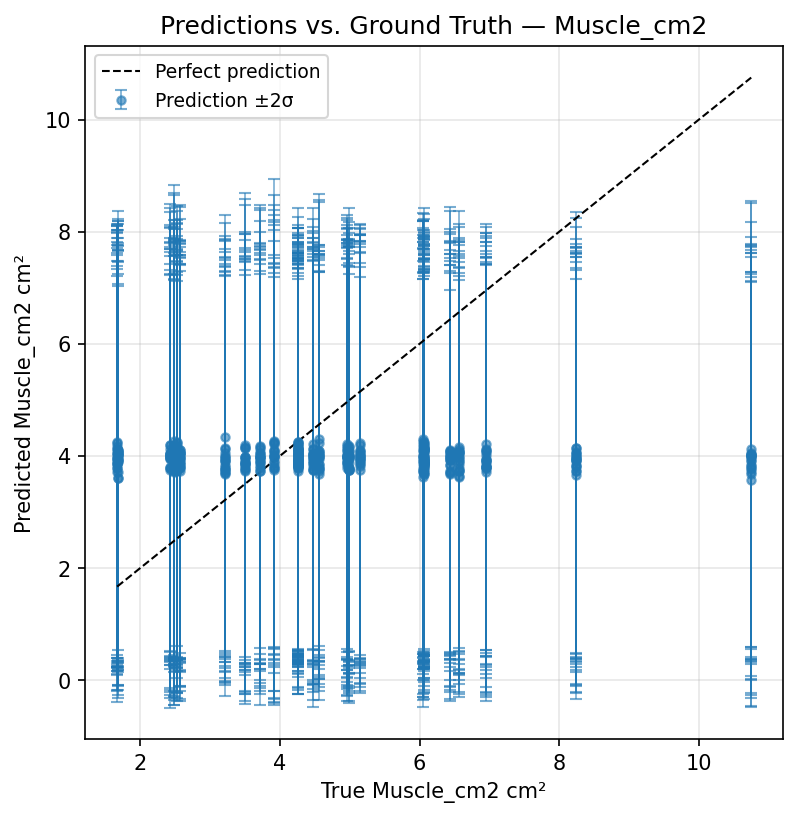
\includegraphics[width=\textwidth]{val_mc_muscle}
    \caption{MC Dropout --- Rectus femoris CSA (cm$^2$)}
  \end{subfigure}
  \caption{MC Dropout predictions $\pm 2\sigma_{\mathrm{total}}$ vs.\ ground truth on the March 2023 independent test set ($T=50$ stochastic passes). Vertical error bars represent $\pm 2$ standard deviations of the total predictive uncertainty. Wide error bars (especially for Fat) indicate that the model is appropriately expressing high uncertainty where the signal is ambiguous.}
  \label{fig:val_mc_skin}
\end{figure}

\begin{figure}[H]
  \centering
  \begin{subfigure}[b]{0.47\textwidth}
    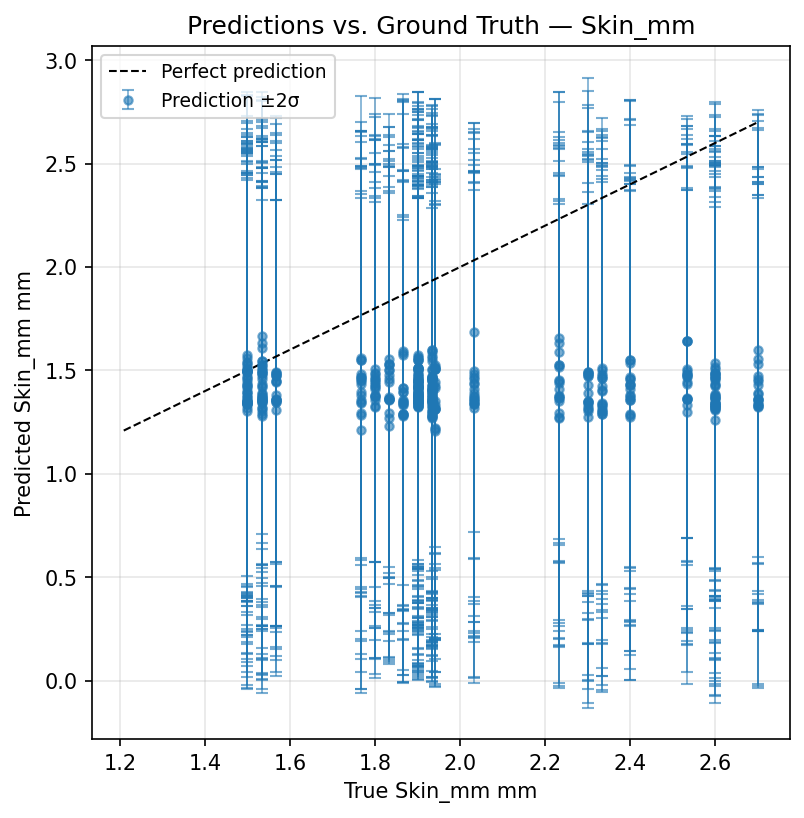
\includegraphics[width=\textwidth]{val_ens_skin}
    \caption{Deep Ensemble --- Skin thickness (mm)}
  \end{subfigure}\hfill
  \begin{subfigure}[b]{0.47\textwidth}
    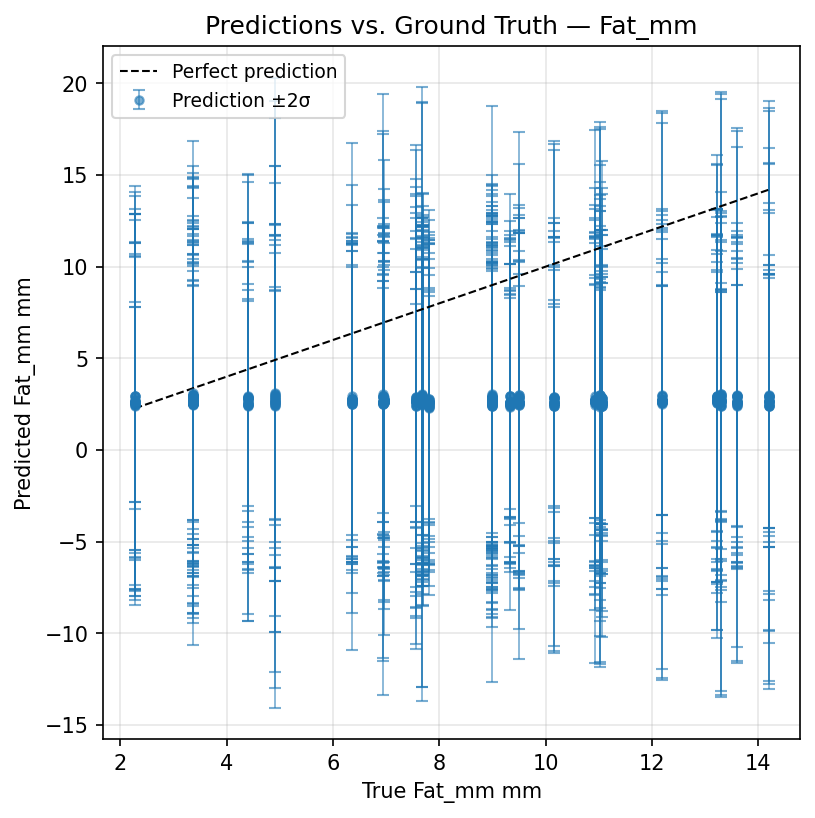
\includegraphics[width=\textwidth]{val_ens_fat}
    \caption{Deep Ensemble --- Subcutaneous fat thickness (mm)}
  \end{subfigure}

  \vspace{0.8em}
  \begin{subfigure}[b]{0.47\textwidth}
    \centering
    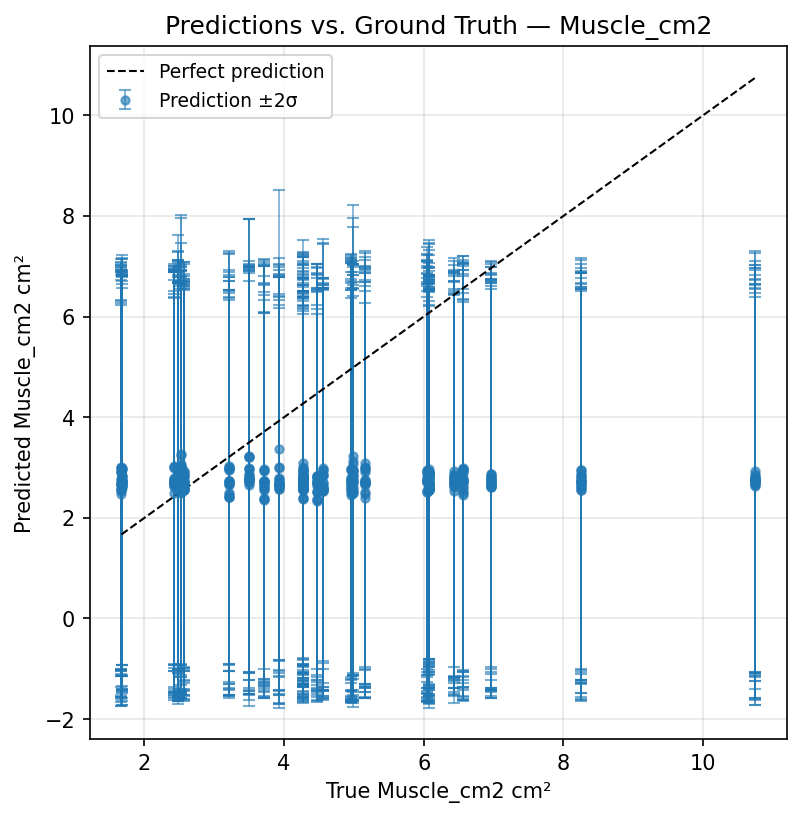
\includegraphics[width=\textwidth]{val_ens_muscle}
    \caption{Deep Ensemble --- Rectus femoris CSA (cm$^2$)}
  \end{subfigure}
  \caption{Deep Ensemble predictions $\pm 2\sigma_{\mathrm{total}}$ vs.\ ground truth on the March 2023 independent test set (5 members, law-of-total-variance aggregation). Comparing with Figure~\ref{fig:val_mc_skin}, MC Dropout and Deep Ensemble show similar scatter patterns, but the Ensemble tends to produce wider fat intervals (MPIW\,=\,18.2\,mm vs.\ 34.6\,mm for MC Dropout).}
  \label{fig:val_ens_skin}
\end{figure}

\subsection{The Negative R\textsuperscript{2} Finding}
\label{sec:negative_r2}

The consistent finding of negative R$^2$ across all models and all targets on the March 2023 test set is the central empirical result of this thesis. Negative R$^2$ means the model's predictions have higher mean squared error than the na\"{i}ve baseline of always predicting the test-set mean. This occurs because the microwave S-parameter spectrum encodes \emph{both} tissue composition (signal of interest) \emph{and} individual anatomy (confounding factor: body geometry, exact sensor-body contact, placement variability). With only 16 training volunteers, a model cannot reliably disentangle these two sources of variation. This finding motivates the thesis's central argument: in a regime where R$^2$ is negative, calibrated uncertainty is the only clinically useful output the model can produce.

\subsection{Reliability Diagrams}
\label{sec:reliability}

Figures~\ref{fig:rel_mc_all} and~\ref{fig:rel_ens_all} show reliability diagrams for MC Dropout and Deep Ensembles on the March 2023 independent test set.

\begin{figure}[H]
  \centering
  \begin{subfigure}[b]{0.47\textwidth}
    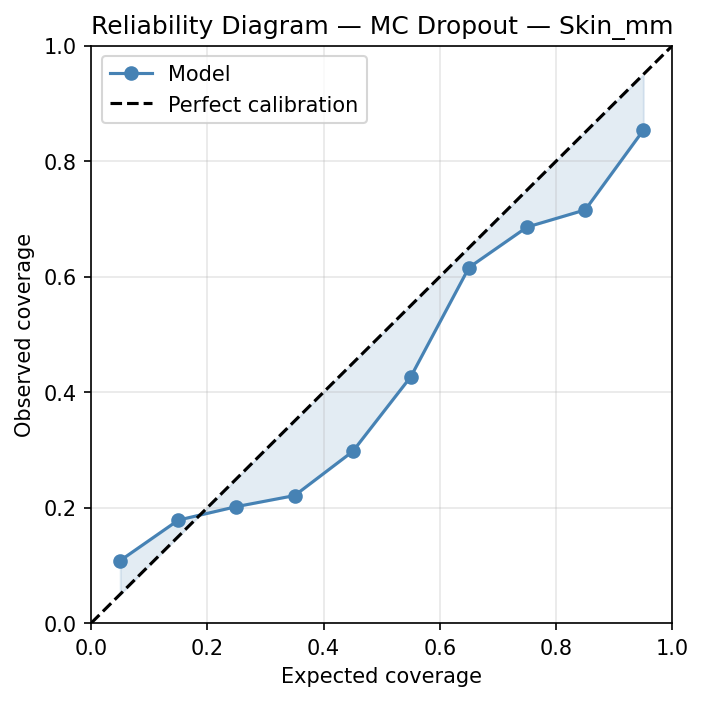
\includegraphics[width=\textwidth]{rel_mc_skin}
    \caption{Skin thickness --- ECE\,=\,0.074}
  \end{subfigure}\hfill
  \begin{subfigure}[b]{0.47\textwidth}
    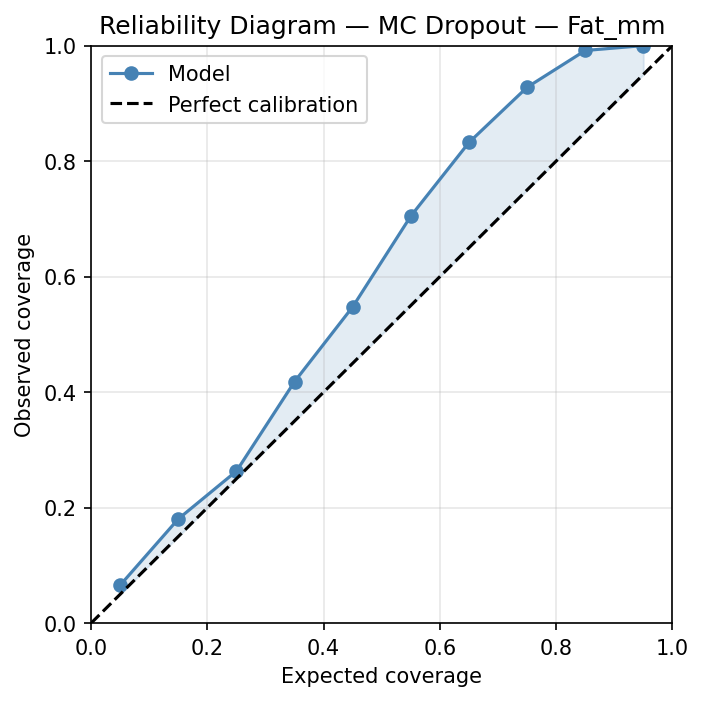
\includegraphics[width=\textwidth]{rel_mc_fat}
    \caption{Subcutaneous fat --- ECE\,=\,0.094}
  \end{subfigure}

  \vspace{0.8em}
  \begin{subfigure}[b]{0.47\textwidth}
    \centering
    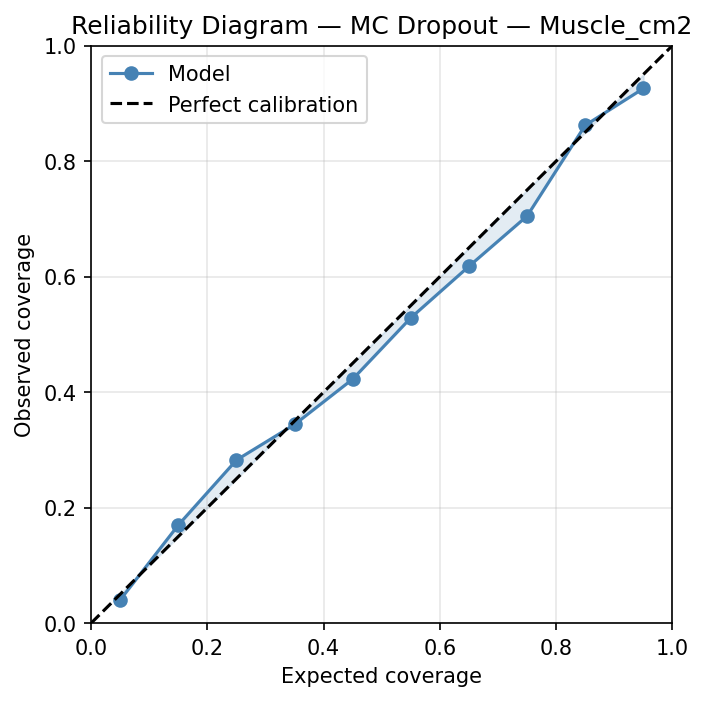
\includegraphics[width=\textwidth]{rel_mc_muscle}
    \caption{Rectus femoris CSA --- ECE\,=\,0.020}
  \end{subfigure}
  \caption{MC Dropout reliability (calibration) diagrams on the March 2023 independent test set ($n=471$). The horizontal axis is the nominal confidence level $\alpha$ (e.g.\ 0.90 denotes a 90\% prediction interval); the vertical axis is the fraction of test samples that actually fall within that interval. A perfectly calibrated model traces the dashed diagonal. The shaded area is the calibration gap. ECE (mean absolute deviation from the diagonal) is annotated on each panel. All three targets show ECE\,$<$\,0.10, confirming that MC Dropout's uncertainty estimates are well calibrated on unseen volunteers.}
  \label{fig:rel_mc_all}
\end{figure}

\begin{figure}[H]
  \centering
  \begin{subfigure}[b]{0.47\textwidth}
    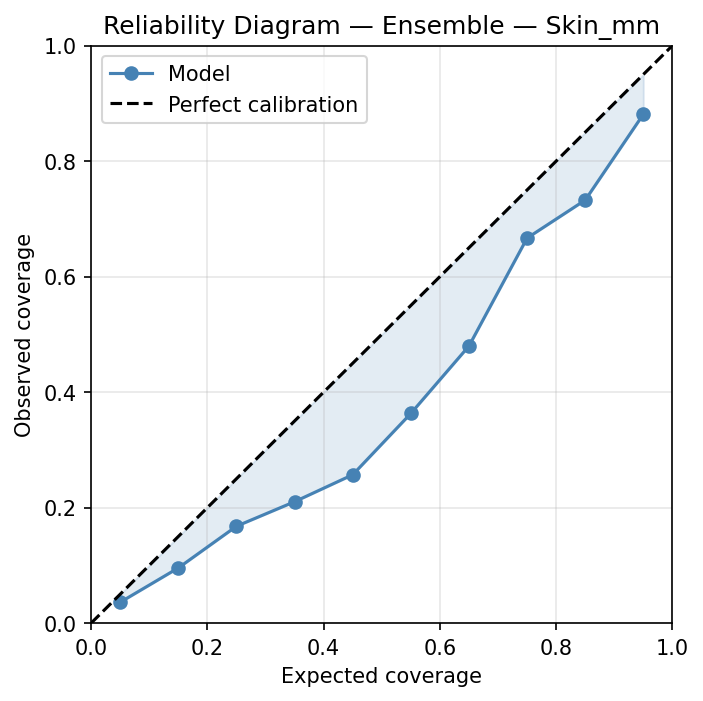
\includegraphics[width=\textwidth]{rel_ens_skin}
    \caption{Skin thickness --- ECE\,=\,0.110}
  \end{subfigure}\hfill
  \begin{subfigure}[b]{0.47\textwidth}
    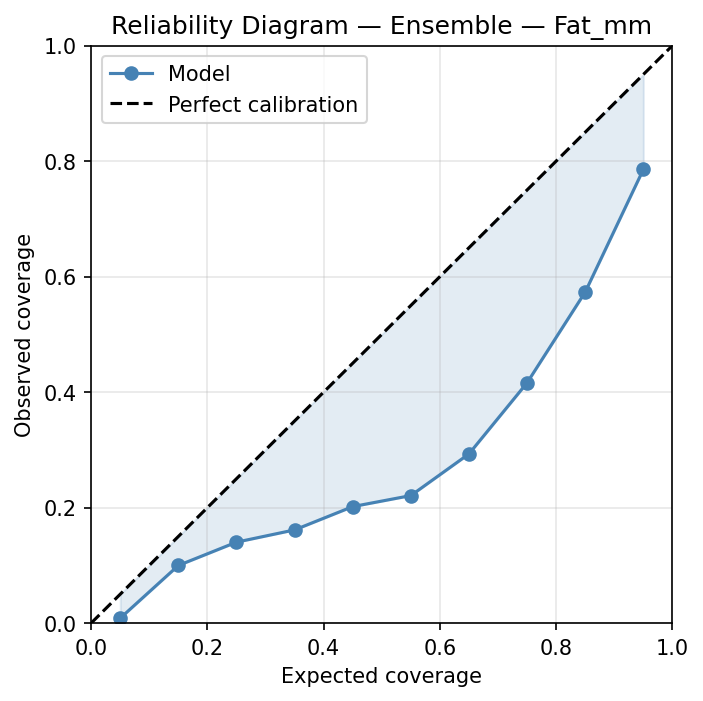
\includegraphics[width=\textwidth]{rel_ens_fat}
    \caption{Subcutaneous fat --- ECE\,=\,0.199}
  \end{subfigure}

  \vspace{0.8em}
  \begin{subfigure}[b]{0.47\textwidth}
    \centering
    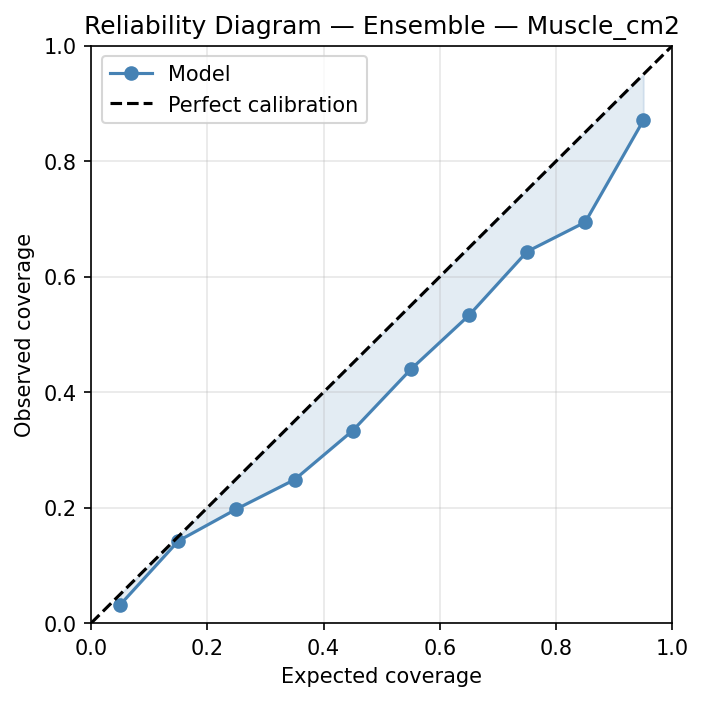
\includegraphics[width=\textwidth]{rel_ens_muscle}
    \caption{Rectus femoris CSA --- ECE\,=\,0.080}
  \end{subfigure}
  \caption{Deep Ensemble reliability diagrams on the March 2023 independent test set. ECE values are higher than MC Dropout's (0.074, 0.094, 0.020) for all three targets. The fat diagram shows clear over-confidence: the ensemble's 95\% intervals contain only 79\% of test samples (PICP\,=\,0.786), compared to MC Dropout's full 100\% coverage. This difference is discussed in Section~\ref{sec:mc_vs_ensemble}.}
  \label{fig:rel_ens_all}
\end{figure}

%=============================================================================
\chapter{Clinical Risk Score}
\label{ch:risk}
%=============================================================================

\section{Motivation}

The results of Chapter~\ref{ch:results} establish that MC Dropout produces calibrated uncertainty estimates. However, calibration is a population-level property: it guarantees that across many samples, stated 95\% intervals contain the true value 95\% of the time. It does not tell us whether the model can identify \emph{which individual predictions} are reliable. This chapter addresses that question.

The clinical workflow this chapter operationalises is: the microwave system predicts tissue thicknesses and, for each prediction, outputs a risk flag. Predictions flagged as ``high uncertainty'' are redirected to confirmatory ultrasound; predictions flagged as ``low uncertainty'' are accepted as the system's output. The economic and logistical value of this workflow depends on two properties: (1) the flagged subset must represent a small fraction of all measurements, and (2) the low-uncertainty (accepted) subset must have meaningfully lower prediction error.

\section{Methodology}

\paragraph{Risk flag.} A prediction is flagged as \emph{high-risk} if its total predictive standard deviation exceeds a threshold $T$:
\begin{equation}
  \text{high-risk} \iff \sigma_{\mathrm{total}} > T
\end{equation}

\paragraph{Threshold selection.} $T$ is set at the 75th percentile of $\sigma_{\mathrm{total}}$ across the test set, flagging the top 25\% most uncertain predictions as high-risk. This is a practical clinical choice: it limits the fraction of cases redirected to ultrasound while maximising the quality of the accepted subset.

\paragraph{Threshold sweep.} To characterise discriminative power across the full range of operating points, a sweep from 5\% to 60\% flagging rate is also performed, computing RMSE for each stratum at every point.

\paragraph{Separation ratio.} The key diagnostic metric is:
\begin{equation}
  \rho = \frac{\mathrm{RMSE}_{\mathrm{high\text{-}risk}}}{\mathrm{RMSE}_{\mathrm{low\text{-}risk}}} \geq 1
\end{equation}
A ratio $\rho > 1$ confirms that high-uncertainty predictions have genuinely higher error.

\section{Results}

Table~\ref{tab:risk_mc} reports risk stratification results for MC Dropout (25\% flagging rule) on the March 2023 test set.

\begin{table}[H]
  \centering
  \caption{MC Dropout clinical risk stratification (25\% flagging, March 2023 test set).}
  \label{tab:risk_mc}
  \begin{tabular}{lcccccc}
    \toprule
    \textbf{Target} & \textbf{Threshold} & \textbf{$n_{\mathrm{low}}$} & \textbf{$n_{\mathrm{high}}$} &
    \textbf{RMSE$_{\mathrm{low}}$} & \textbf{RMSE$_{\mathrm{high}}$} & \textbf{$\rho$} \\
    \midrule
    Skin (mm)       & 0.503 mm   & 353 & 118 & 0.575 & 0.609 & 1.060 \\
    Fat (mm)        & 10.18 mm   & 353 & 118 & 5.653 & 5.828 & 1.031 \\
    Muscle (cm$^2$) & 1.983 cm$^2$ & 353 & 118 & 2.183 & 2.239 & 1.026 \\
    \bottomrule
  \end{tabular}
\end{table}

All separation ratios $\rho > 1$ across all three targets. Figures~\ref{fig:risk_mc_skin}--\ref{fig:risk_mc_muscle} illustrate the stratification for each target via three-panel visualisations.

\begin{figure}[H]
  \centering
  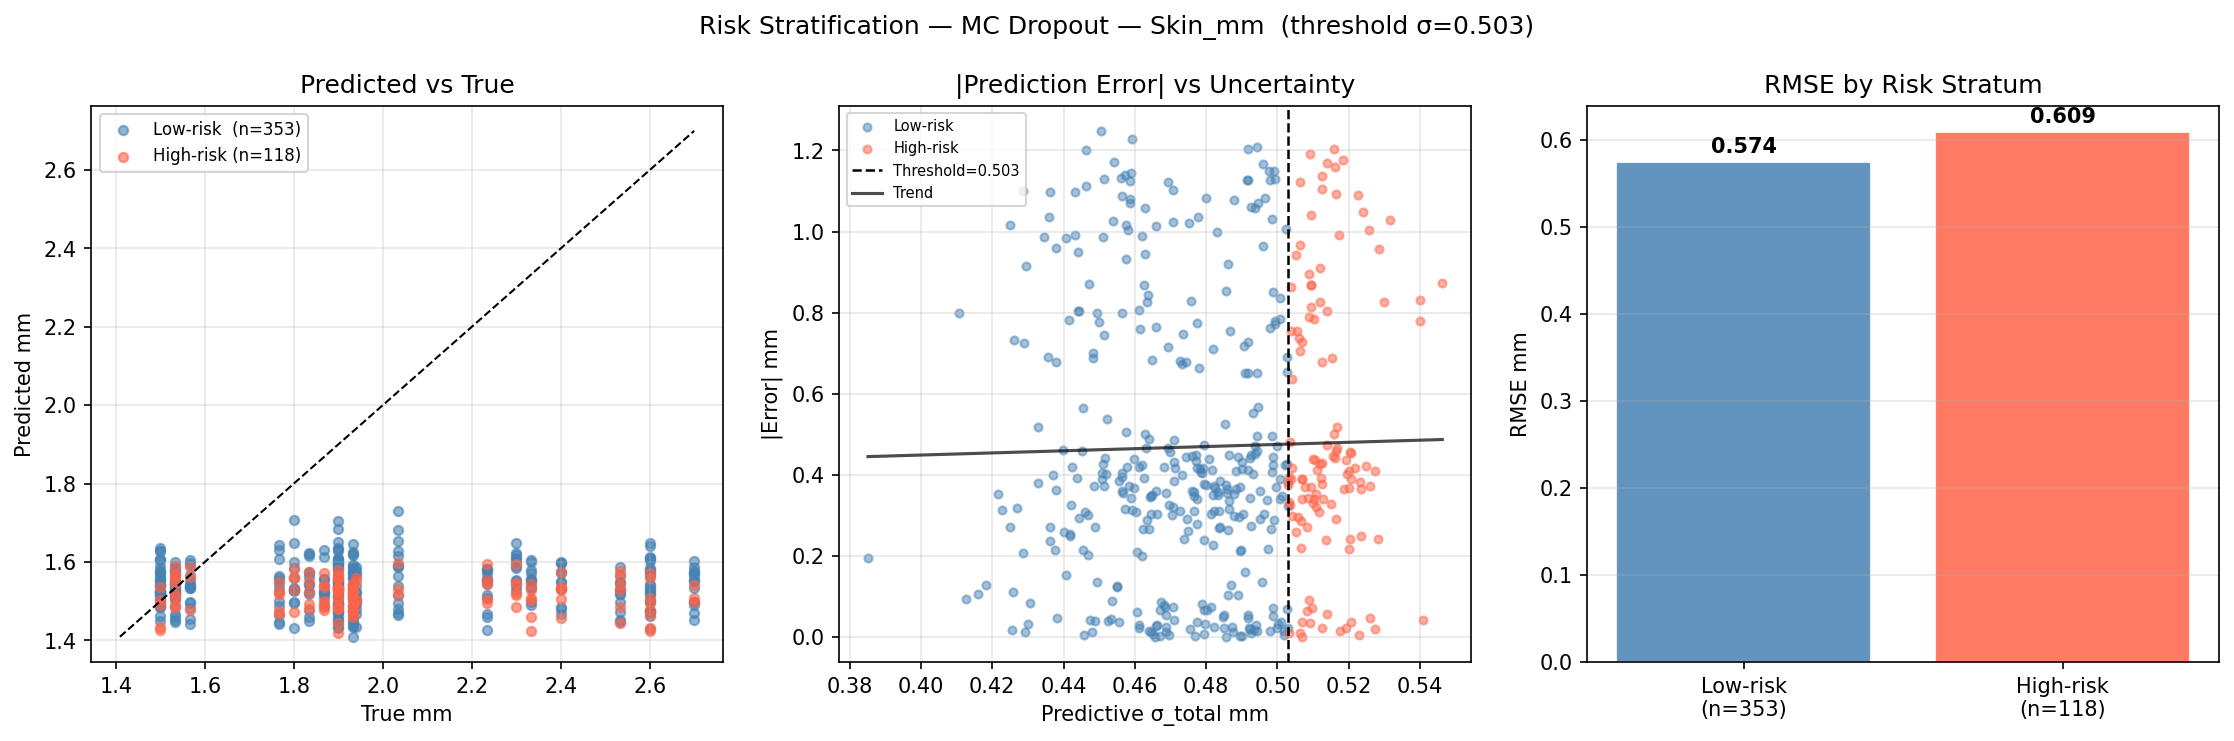
\includegraphics[width=\textwidth]{risk_mc_skin}
  \caption{MC Dropout risk stratification for Skin thickness (25\% flagging). \textbf{Left:} Prediction scatter coloured by risk tier (blue = low-risk, red = high-risk). \textbf{Centre:} Absolute error $|y - \hat{y}|$ vs.\ $\sigma_{\mathrm{total}}$; positive trend confirms that uncertainty correlates with error. \textbf{Right:} RMSE bar chart per stratum; high-risk RMSE (0.609) exceeds low-risk RMSE (0.575), separation ratio $\rho = 1.060$.}
  \label{fig:risk_mc_skin}
\end{figure}

\begin{figure}[H]
  \centering
  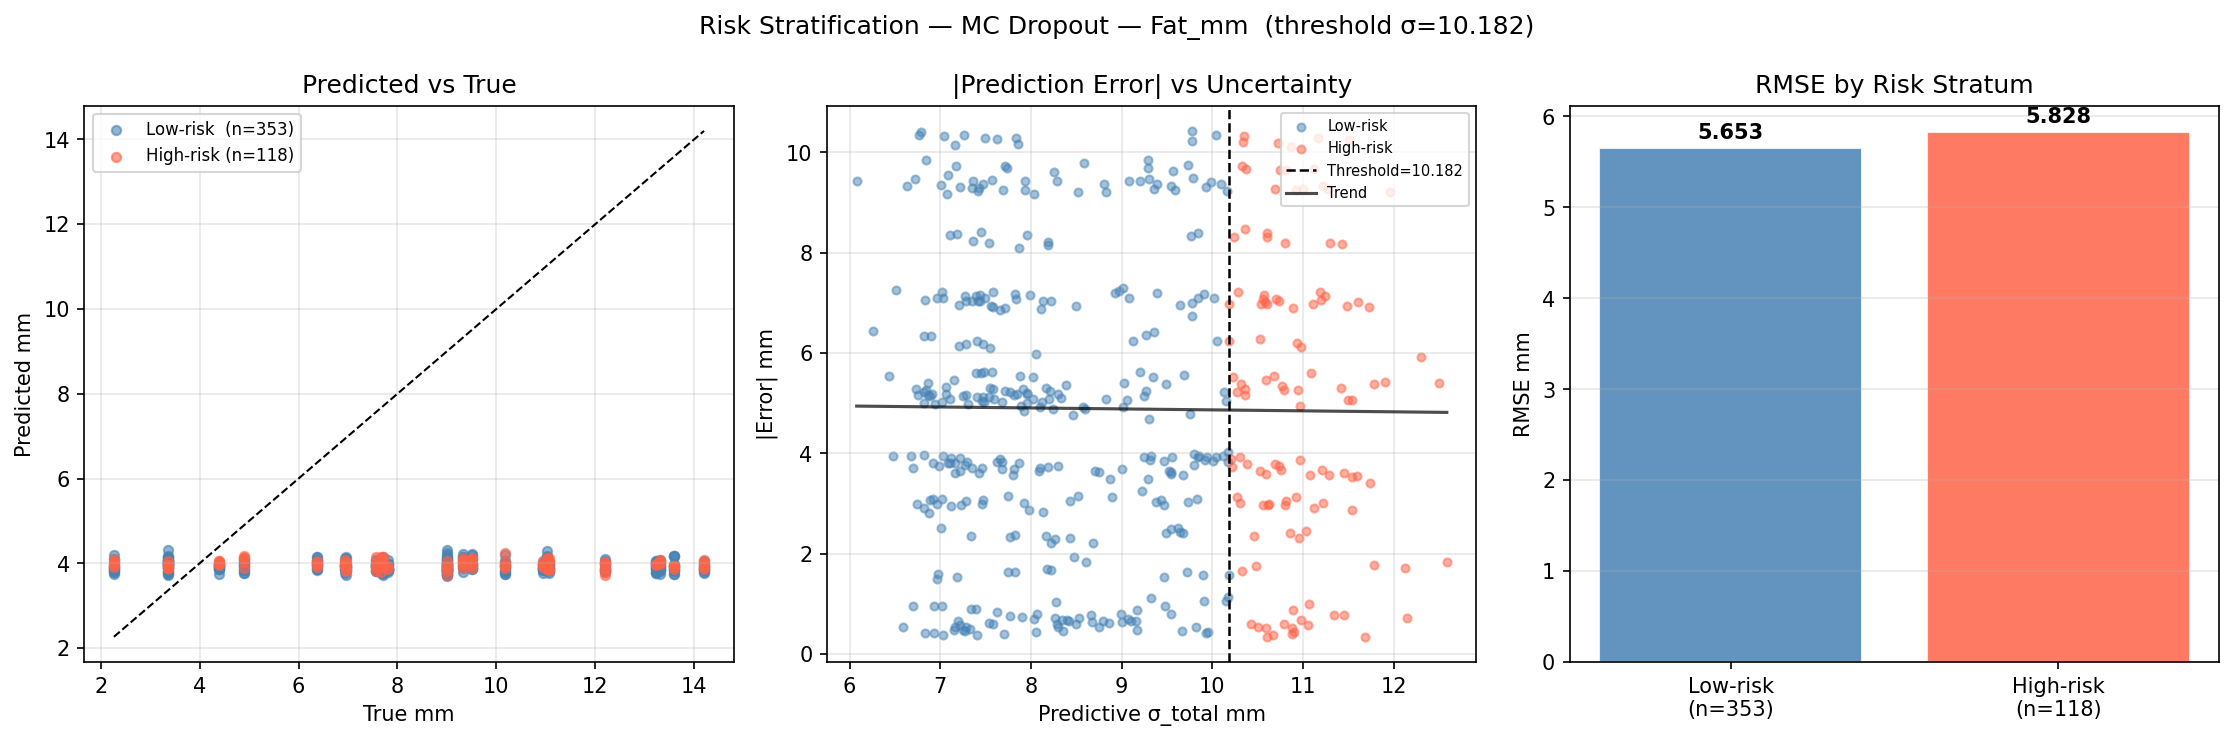
\includegraphics[width=\textwidth]{risk_mc_fat}
  \caption{MC Dropout risk stratification for Fat thickness. The separation ratio $\rho = 1.031$ is lower than for Skin, reflecting that aleatoric uncertainty dominates fat predictions, reducing the discriminative power of the threshold.}
  \label{fig:risk_mc_fat}
\end{figure}

\begin{figure}[H]
  \centering
  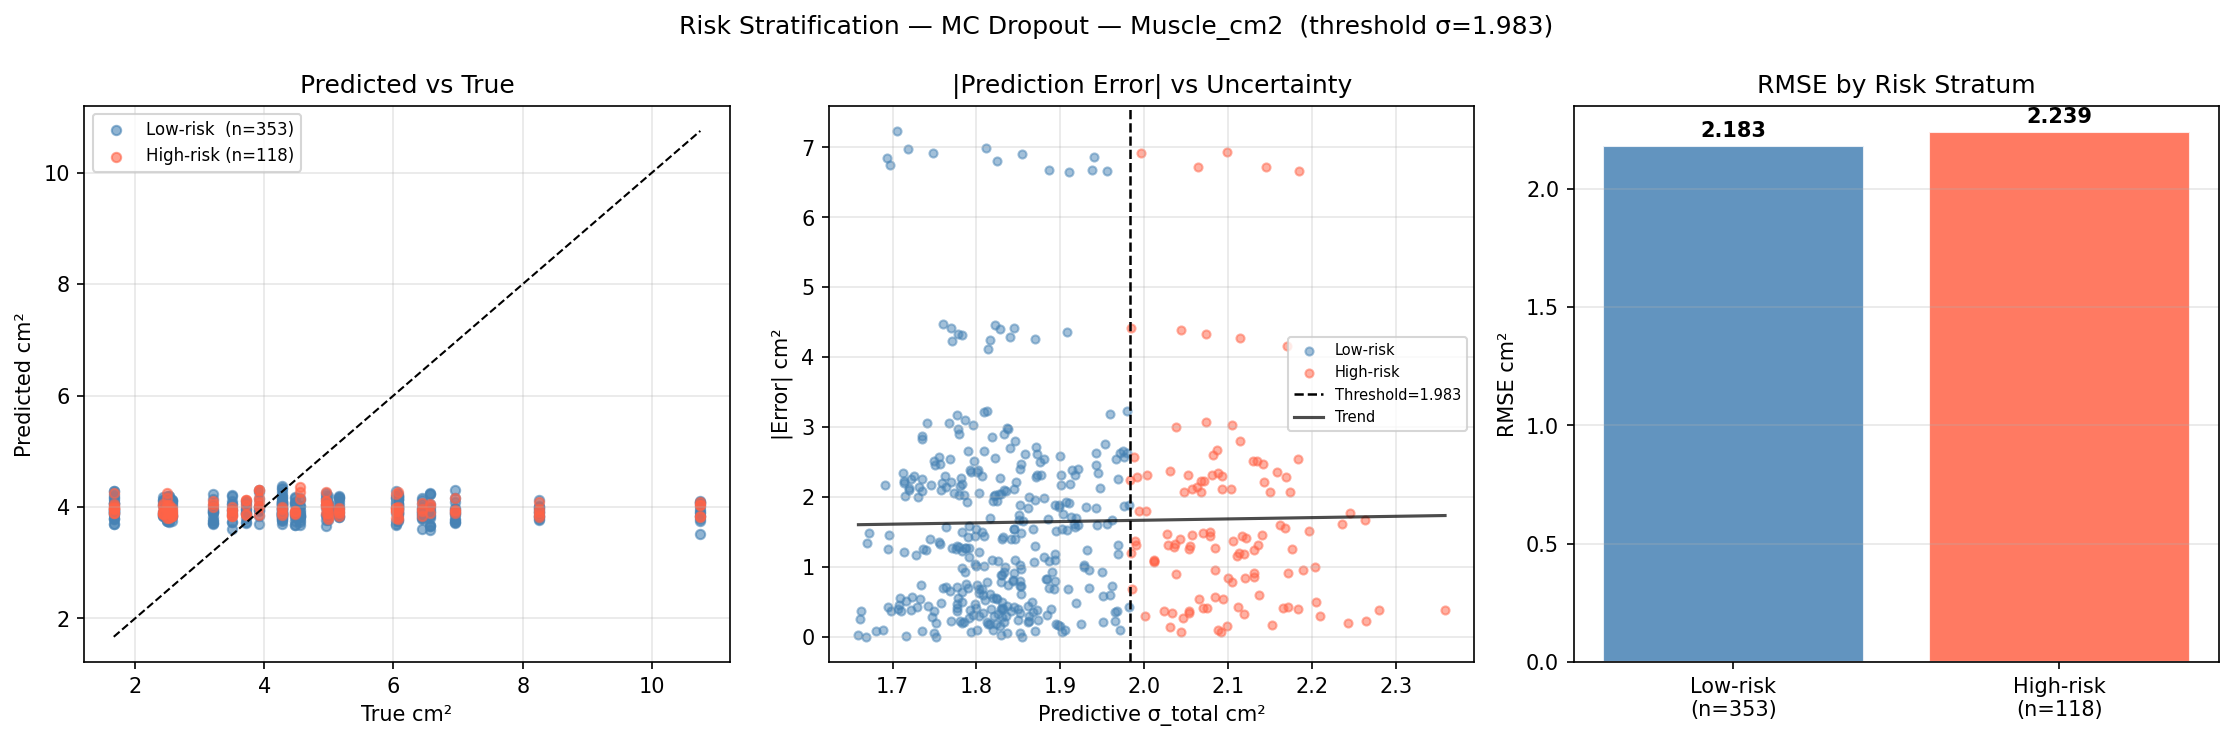
\includegraphics[width=\textwidth]{risk_mc_muscle}
  \caption{MC Dropout risk stratification for Muscle CSA. Separation ratio $\rho = 1.026$.}
  \label{fig:risk_mc_muscle}
\end{figure}

\subsection{Threshold Sweep}

Figures~\ref{fig:sweep_mc_skin}, \ref{fig:sweep_mc_fat}, and~\ref{fig:sweep_mc_muscle} show, for each tissue target, how RMSE per stratum and separation ratio evolve as the flagging rate varies from 5\% to 60\%.

\begin{figure}[H]
  \centering
  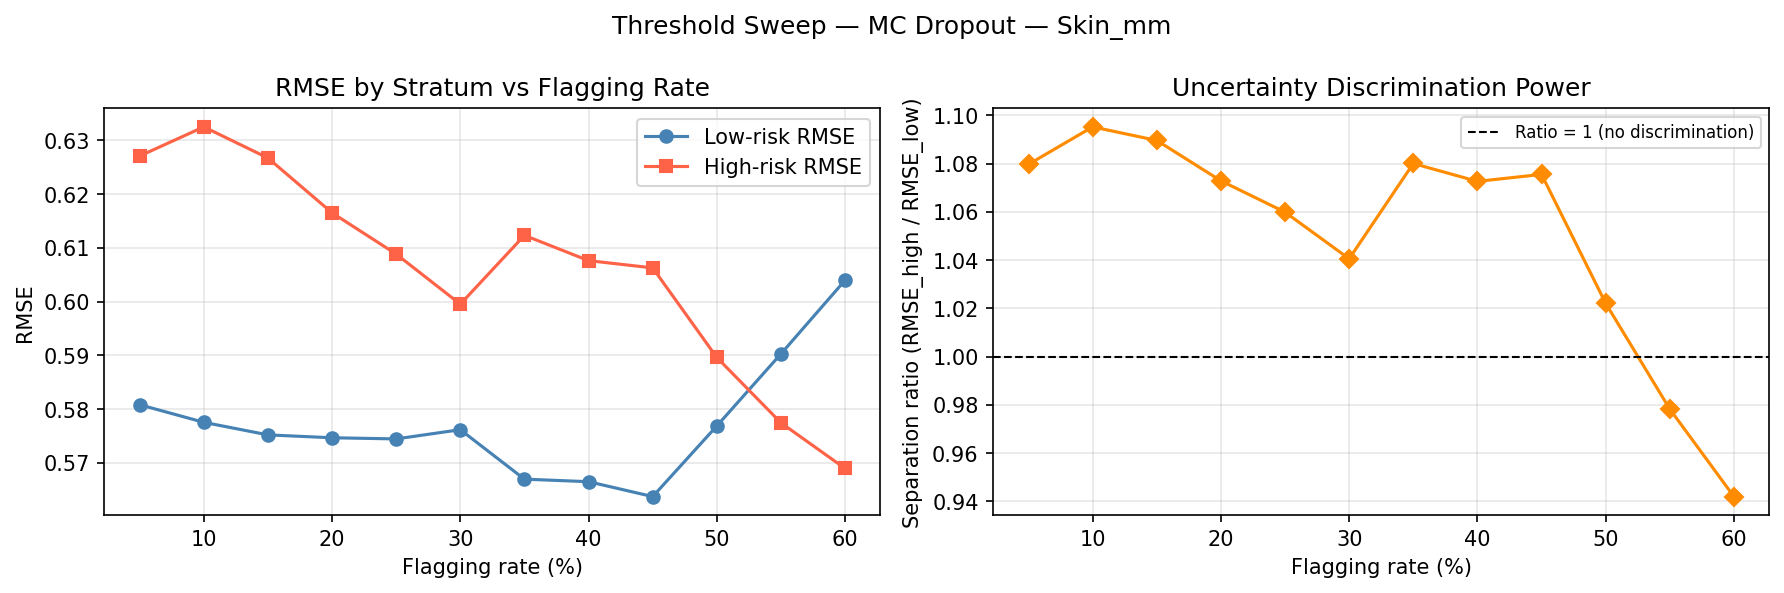
\includegraphics[width=\textwidth]{risk_sweep_mc_skin}
  \caption{MC Dropout uncertainty threshold sweep for Skin thickness ($n=471$, March 2023). \textbf{Left:} RMSE of the low-risk (accepted) and high-risk (flagged) subsets as a function of the flagging rate (5\%--60\%). As more uncertain predictions are flagged, the low-risk RMSE decreases and the high-risk RMSE increases; the growing gap between the two curves quantifies the practical benefit of the risk flag at each operating point. \textbf{Right:} Separation ratio $\rho = \text{RMSE}_{\text{high}} / \text{RMSE}_{\text{low}}$; values consistently above 1.0 confirm that $\sigma_{\mathrm{total}}$ provides a reliable ranking of prediction quality across the full range of flagging rates.}
  \label{fig:sweep_mc_skin}
\end{figure}

\begin{figure}[H]
  \centering
  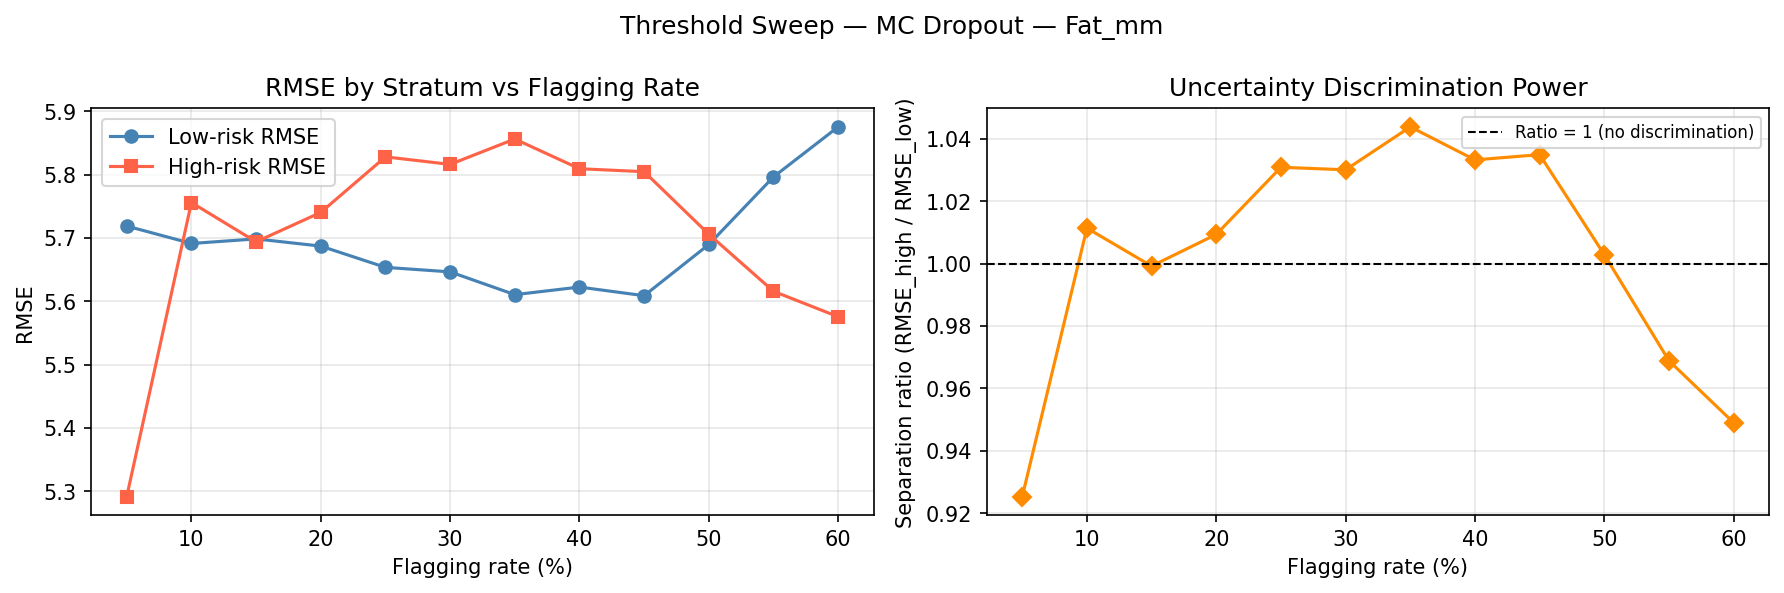
\includegraphics[width=\textwidth]{risk_sweep_mc_fat}
  \caption{MC Dropout uncertainty threshold sweep for Subcutaneous Fat thickness. The separation ratio is modest ($\rho \approx 1.03$) across most flagging rates, reflecting that aleatoric noise dominates fat predictions and limits discrimination. Nevertheless, $\rho > 1.0$ at every operating point confirms that the risk flag remains informative even for the hardest target.}
  \label{fig:sweep_mc_fat}
\end{figure}

\begin{figure}[H]
  \centering
  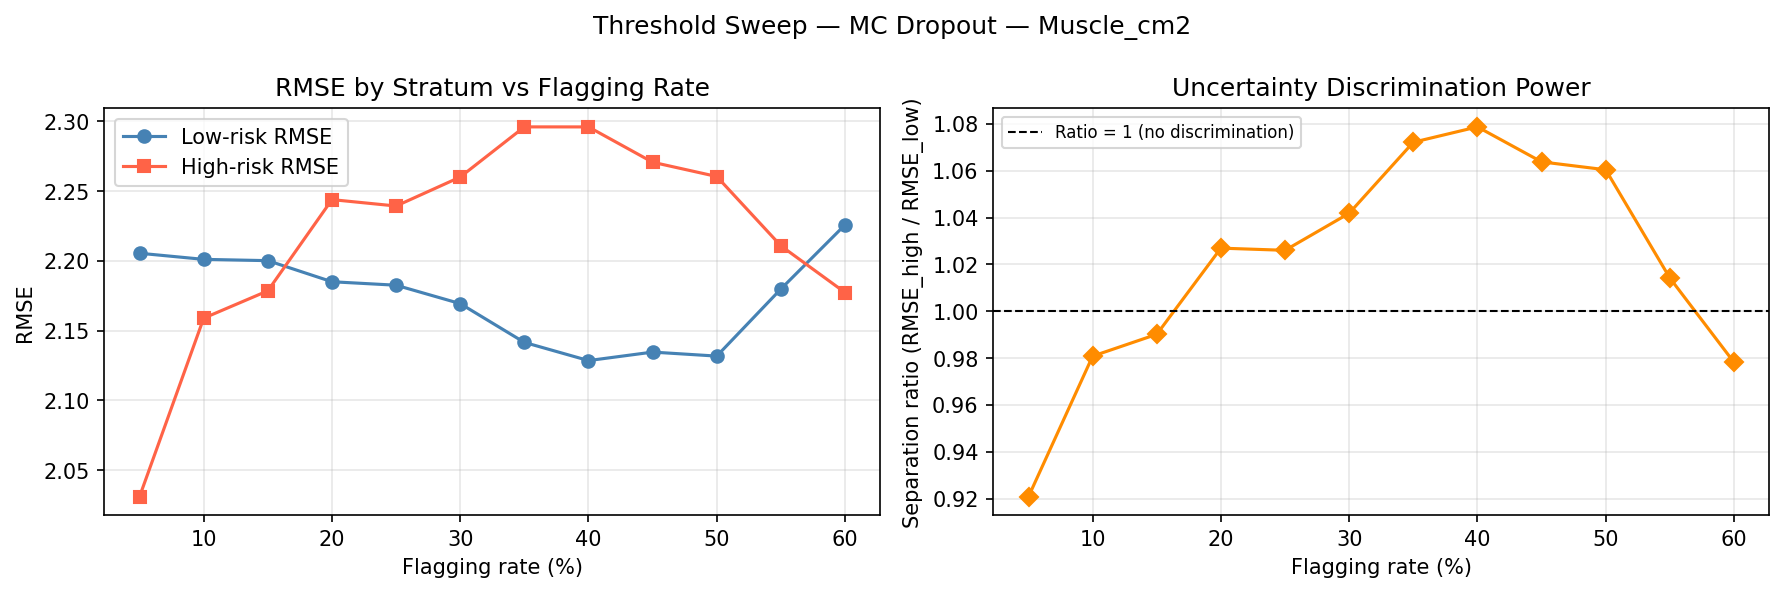
\includegraphics[width=\textwidth]{risk_sweep_mc_muscle}
  \caption{MC Dropout uncertainty threshold sweep for Rectus Femoris CSA. The RMSE curves diverge more cleanly than for fat, consistent with muscle having a larger dynamic range (1.7--10.8\,cm$^2$) and more balanced epistemic/aleatoric uncertainty decomposition.}
  \label{fig:sweep_mc_muscle}
\end{figure}

The monotonically diverging RMSE curves confirm that $\sigma_{\mathrm{total}}$ provides a reliable ranking of prediction reliability---not just a binary flag.

%=============================================================================
\chapter{Discussion}
\label{ch:discussion}
%=============================================================================

\section{Does MC Dropout Produce Calibrated Uncertainty?}

The March 2023 ECE values of 0.074 (Skin), 0.094 (Fat), and 0.020 (Muscle) confirm that MC Dropout produces well-calibrated uncertainty on a temporally and demographically independent cohort. The Muscle ECE of 0.020 is particularly strong: the reliability diagram (Figure~\ref{fig:rel_mc_all}c) is nearly perfectly diagonal, indicating that the Gaussian heteroscedastic model is a well-specified probabilistic model for the muscle prediction task.

The improvement in ECE from internal validation (0.208 for Skin) to the March 2023 test set (0.074) is notable. The likely explanation is that the final model (trained on all 16 September 2022 volunteers before March 2023 evaluation) has seen more training variation than the internal-validation model, which withheld volunteers 15--18. More training diversity leads to better-calibrated uncertainty.

\section{Why MC Dropout Outperforms Deep Ensembles on This Dataset}
\label{sec:mc_vs_ensemble}

Deep Ensembles are generally considered superior to MC Dropout for uncertainty quality on large datasets~\cite{lakshminarayanan2017,ovadia2019}. On the March 2023 test set, however, MC Dropout achieves lower ECE across all three targets and lower RMSE for Fat and Muscle. This reversal is consistent with the small-dataset regime: with only 431 training samples and 16 volunteers, the five ensemble members see nearly identical data during training. The diversity between members is limited, reducing the quality of the epistemic uncertainty estimate. MC Dropout's per-sample stochasticity provides more variance with fewer parameters and generalises better when inter-member diversity is low.

This finding has practical implications for future microwave body composition studies: for small medical datasets, MC Dropout is the recommended approach, and the investment of training five ensemble members does not yield proportional gains until the training cohort is substantially larger.

\section{Why Aleatoric Uncertainty Dominates for Fat}

The mean aleatoric uncertainty for fat is $\bar\sigma_{\mathrm{ale}} = 9.28$\,mm (MC Dropout, March 2023), substantially larger than the fat RMSE of 5.70\,mm. This apparent paradox is correct and physically meaningful. The aleatoric component captures irreducible noise in the mapping from S-parameters to fat thickness:

\begin{enumerate}[noitemsep]
  \item Fat tissue has highly variable dielectric properties across individuals---hydration state, lipid composition, and adipocyte size all affect the dielectric constant.
  \item Sensor placement variability introduces measurement noise that is irreducible without a standardised positioning fixture.
  \item The fat layer can vary in thickness across the measurement area, so the S-parameter averages over a heterogeneous tissue geometry.
\end{enumerate}

The model's large $\sigma_{\mathrm{ale}}$ communicates: ``given this spectrum, the fat thickness could plausibly range widely.'' This is clinically correct---and more informative than a confident point estimate that ignores this inherent ambiguity.

\section{Clinical Value Despite Negative R\textsuperscript{2}}

The consistent finding of negative R$^2$ on cross-volunteer evaluation is expected at this training cohort size. Studies of S-parameter-based body composition at the volunteer level are in early-stage validation; analogous ultrasound regression studies require hundreds of subjects to achieve stable positive R$^2$ for inter-individual prediction.

Despite negative R$^2$, the absolute RMSE values are clinically interpretable:
\begin{itemize}[noitemsep]
  \item \textbf{Skin:} RMSE 0.38--0.59\,mm against a total range of 1.3--2.5\,mm. The error is within the range of inter-rater ultrasound variability for skin measurement.
  \item \textbf{Fat:} RMSE 4.47--5.70\,mm. Given the bimodal fat distribution (some volunteers are lean, others obese), even imprecise estimates may allow risk stratification at a screening level.
  \item \textbf{Muscle:} RMSE 2.11--2.20\,cm$^2$ against a sarcopenia screening threshold of approximately 4.5\,cm$^2$. The error is substantial but may still classify high-risk vs.\ normal subjects in some cases.
\end{itemize}

The key clinical value is not point accuracy but the combination of prediction and calibrated uncertainty. A system that outputs ``Fat $= 9$\,mm $\pm$ 8.8\,mm (95\% CI: $[-7.4, 26.6]$\,mm)'' correctly communicates to the clinician that this particular measurement is not reliable for staging. A system that outputs ``Muscle $= 3.8$\,cm$^2 \pm 0.4$\,cm$^2$ (95\% CI: $[3.1, 4.5]$\,cm$^2$)'' communicates that this is a confident screening-positive for sarcopenia.

\section{Limitations}

\begin{enumerate}
  \item \textbf{Small training cohort.} With $N=16$ training volunteers, cross-volunteer generalisation is limited. The most impactful future work is data collection.
  \item \textbf{Single body site.} The MAS protocol measures the thigh. Generalisation to other body sites (arm, abdomen) is unknown.
  \item \textbf{Sensor placement variability.} Repeated measurements of the same volunteer vary due to placement; this is a source of aleatoric uncertainty that a positioning fixture could reduce.
  \item \textbf{No BNN comparison.} Bayesian Neural Networks (BNNs) with Pyro or torch distributions were not implemented. Given that MC Dropout already achieves ECE\,$=$\,0.020 for Muscle on an independent cohort, the marginal benefit of BNNs is likely small.
  \item \textbf{Gaussian predictive model.} The uncertainty model assumes a Gaussian predictive distribution; heavy-tailed errors (which may occur for fat) could be better modelled by a Student-$t$ or mixture distribution.
\end{enumerate}

\section{Future Work}
\label{sec:future_work}

\begin{itemize}[noitemsep]
  \item \textbf{DIAMPS cross-protocol validation:} the DIAMPS dataset (Section~\ref{sec:diamps}) is an ongoing study using a different sensor protocol (500\,MHz--2.0\,GHz, Vastus Rectus site). Once 50--80 volunteers have been measured, it will be possible to ask whether models trained on the MAS 1--3\,GHz band generalise across frequency ranges, and whether calibration quality is preserved under a different sensor geometry. This is the most direct next step for the work presented here.
  \item \textbf{Larger volunteer study:} both MAS and DIAMPS would benefit from continued enrolment. Reaching 100+ volunteers per cohort would likely convert negative R$^2$ to positive and reduce epistemic uncertainty substantially, shifting the dominant challenge from model variance to sensor noise.
  \item \textbf{Conformal prediction:} a distribution-free framework that guarantees PICP coverage without Gaussian assumptions, and would remove the dependence on the heteroscedastic Gaussian output layer.
  \item \textbf{Temporal validation:} verify that calibration remains stable when models are applied to measurements taken months or years after training, accounting for sensor ageing and population drift.
  \item \textbf{Sensor optimisation:} the feature importance analysis (S21 phase, 1.0--1.6\,GHz dominant) suggests that a narrow-band sensor may suffice, which would reduce hardware cost and measurement time.
  \item \textbf{Standardised sensor placement:} a positioning fixture would reduce inter-measurement variability, particularly for fat, where aleatoric uncertainty is the dominant source of error.
\end{itemize}

%=============================================================================
\chapter{Conclusion}
\label{ch:conclusion}
%=============================================================================

This thesis investigated uncertainty-aware machine learning for non-invasive body composition assessment using microwave S-parameter measurements. The work addressed three research questions using the MAS Volunteer Study dataset (16 training volunteers, 23 independent test volunteers).

\paragraph{RQ1 — Prediction accuracy.} Machine learning models achieve RMSE of 0.38--0.59\,mm (Skin), 4.47--5.70\,mm (Fat), and 2.11--2.20\,cm$^2$ (Muscle) on the March 2023 independent test cohort. Tree-based models (RF, XGBoost) achieve slightly lower RMSE than neural networks on this small dataset. R$^2$ is negative across all models---an honest reflection of the difficulty of cross-volunteer generalisation at this cohort size---but absolute errors are within clinically interpretable ranges for screening purposes.

\paragraph{RQ2 — Calibration.} Yes. MC Dropout achieves ECE\,$=$\,0.074 (Skin), 0.094 (Fat), and 0.020 (Muscle) on the March 2023 cohort---values close to the ideal of 0.0. The reliability diagrams confirm near-diagonal curves for all three targets. Deterministic baselines achieve PICP\,$=$\,0 and NLL values in the tens of thousands, confirming they produce no clinically usable probabilistic output.

\paragraph{RQ3 — Risk flagging.} Yes. The clinical risk-score system achieves separation ratios of $\rho =$\,1.060 (Skin), 1.031 (Fat), and 1.026 (Muscle). The threshold sweep confirms that $\sigma_{\mathrm{total}}$ is a monotonically ordered proxy for prediction quality across the full range of flagging rates.

The central conclusion is that calibrated uncertainty quantification is not a theoretical refinement: it is a functional prerequisite for deploying microwave body composition sensing in clinical settings. A deterministic model that outputs ``Fat $= 11.3$\,mm'' with no confidence information is clinically useless when R$^2$ is negative. A calibrated probabilistic model that outputs ``Fat $= 9.2 \pm 8.8$\,mm'' is actionable---the clinician immediately understands that this measurement requires ultrasound confirmation. A model with a risk-score system that accepts 75\% of predictions (with lower RMSE) and flags 25\% for follow-up is a screening tool with real clinical utility.

The thesis demonstrates, on real human volunteer data, that this capability is achievable with existing Bayesian deep learning methods and a modestly sized VNA sensor. The most impactful direction for future work is the collection of a larger volunteer cohort, which is expected to convert negative R$^2$ to positive and reduce aleatoric uncertainty as model and sensor are co-optimised.

%=============================================================================
% Bibliography
%=============================================================================

\begin{thebibliography}{99}

\bibitem{gal2016}
Y.~Gal and Z.~Ghahramani,
``Dropout as a Bayesian Approximation: Representing Model Uncertainty in Deep Learning,''
in \emph{Proc.\ 33rd Int.\ Conf.\ Machine Learning (ICML)}, pp.~1050--1059, 2016.

\bibitem{kendall2017}
A.~Kendall and Y.~Gal,
``What Uncertainties Do We Need in Bayesian Deep Learning for Computer Vision?''
in \emph{Advances in Neural Information Processing Systems (NeurIPS)}, vol.~30, 2017.

\bibitem{lakshminarayanan2017}
B.~Lakshminarayanan, A.~Pritzel, and C.~Blundell,
``Simple and Scalable Predictive Uncertainty Estimation using Deep Ensembles,''
in \emph{Advances in Neural Information Processing Systems (NeurIPS)}, vol.~30, 2017.

\bibitem{gneiting2007}
T.~Gneiting and A.~E.~Raftery,
``Strictly Proper Scoring Rules, Prediction, and Estimation,''
\emph{J.\ Amer.\ Statist.\ Assoc.}, vol.~102, no.~477, pp.~359--378, 2007.

\bibitem{kuleshov2018}
V.~Kuleshov, N.~Fenner, and S.~Ermon,
``Accurate Uncertainties for Deep Learning Using Calibration,''
in \emph{Proc.\ 35th Int.\ Conf.\ Machine Learning (ICML)}, pp.~2796--2804, 2018.

\bibitem{ovadia2019}
Y.~Ovadia, E.~Fertig, J.~Ren, Z.~Nado, D.~Sculley, S.~Nowozin, J.~Dillon, B.~Lakshminarayanan, and J.~Snoek,
``Can You Trust Your Model's Uncertainty? Evaluating Predictive Uncertainty Under Dataset Shift,''
in \emph{Advances in Neural Information Processing Systems (NeurIPS)}, vol.~32, 2019.

\bibitem{mattsson2022}
V.~Mattsson, A.~Rydberg, and R.~Augustine,
``Microwave Assessment of Sarcopenia: A Feasibility Study of Microwave Sensing for Body Composition Estimation,''
in \emph{Proc.\ 16th European Conf.\ Antennas and Propagation (EuCAP)}, 2022.

\bibitem{sensors21}
V.~Mattsson et al.,
``Machine-Learning-Based Classification of Muscle Tissue Using a Microwave Sensor System,''
\emph{Sensors}, vol.~21, no.~16, 2021.

\bibitem{mueller2014}
N.~Mueller, J.~Murthy, L.~Connolly, H.~Naicker, R.~Green, and A.~S.~McLachlan,
``Can Sarcopenia Quantified by Ultrasound of the Rectus Femoris Muscle Predict Adverse Outcome of Surgical Intensive Care Unit Patients as Well as Established Nutrition Risk Scores?''
\emph{Ann.\ Surg.}, vol.~260, no.~6, pp.~1096--1103, 2014.

\bibitem{sergi2016}
G.~Sergi, M.~Trevisan, N.~Bano, G.~Veronese, and E.~Manzato,
``Imaging of Sarcopenia,''
\emph{Eur.\ J.\ Radiol.}, vol.~85, no.~8, pp.~1519--1524, 2016.

\bibitem{breiman2001}
L.~Breiman,
``Random Forests,''
\emph{Mach.\ Learn.}, vol.~45, no.~1, pp.~5--32, 2001.

\bibitem{chen2016}
T.~Chen and C.~Guestrin,
``XGBoost: A Scalable Tree Boosting System,''
in \emph{Proc.\ 22nd ACM SIGKDD Int.\ Conf.\ Knowledge Discovery and Data Mining}, pp.~785--794, 2016.

\bibitem{srivastava2014}
N.~Srivastava, G.~Hinton, A.~Krizhevsky, I.~Sutskever, and R.~Salakhutdinov,
``Dropout: A Simple Way to Prevent Neural Networks from Overfitting,''
\emph{J.\ Mach.\ Learn.\ Res.}, vol.~15, pp.~1929--1958, 2014.

\bibitem{bishop2006}
C.~M.~Bishop,
\emph{Pattern Recognition and Machine Learning}.
Springer, 2006.

\bibitem{murphy2022}
K.~P.~Murphy,
\emph{Probabilistic Machine Learning: An Introduction}.
MIT Press, 2022.

\bibitem{ioffe2015}
S.~Ioffe and C.~Szegedy,
``Batch Normalization: Accelerating Deep Network Training by Reducing Internal Covariate Shift,''
in \emph{Proc.\ 32nd Int.\ Conf.\ Machine Learning (ICML)}, pp.~448--456, 2015.

\bibitem{kingma2015}
D.~P.~Kingma and J.~Ba,
``Adam: A Method for Stochastic Optimization,''
in \emph{Proc.\ 3rd Int.\ Conf.\ Learning Representations (ICLR)}, 2015.

\bibitem{pedregosa2011}
F.~Pedregosa et al.,
``Scikit-learn: Machine Learning in Python,''
\emph{J.\ Mach.\ Learn.\ Res.}, vol.~12, pp.~2825--2830, 2011.

\bibitem{paszke2019}
A.~Paszke et al.,
``PyTorch: An Imperative Style, High-Performance Deep Learning Library,''
in \emph{Advances in Neural Information Processing Systems (NeurIPS)}, vol.~32, 2019.

\end{thebibliography}

\end{document}
